%%%%%%%%%%%%%%%%%%%%%%%%%%%%%%%%%%%%%%%%%%%%%%%%%%%%%%%%%%%%%%%%%
% LaTeX Template for 22.106 Notes
% J. Roberts
% Spring, 2011
% Note, requires LATEST version of memoir class 
%%%%%%%%%%%%%%%%%%%%%%%%%%%%%%%%%%%%%%%%%%%%%%%%%%%%%%%%%%%%%%%%%

%---------------------------------------------------------------%
% PREAMBLE
%---------------------------------------------------------------%

\documentclass[ letterpaper, 11pt, twoside, openany ]{memoir}
% NOTE: The option ``oneside'' is for one-sided printing and happens
%       to reduce several blank pages that would otherwise arise.

% This gives a bit more white space...possibly desirable.
%\OnehalfSpace

\usepackage{format106}


%---------------------------------------------------------------%
% DOCUMENT
%---------------------------------------------------------------%

\begin{document}

%%%%%%%%%%%%%%%%%%%%%%%%%%%%%%%%%%%%%%%%%%%%%%%%%%%%%%%%%%%
% Insert Title
\thispagestyle{empty}
\titleTH

\frontmatter
\addtocontents{toc}{\protect\thispagestyle{plain}}
\tableofcontents*

\mainmatter 

\part{Nuclear Data}

\chapter{Microscopic Interactions}
\epigraph{  \begin{SingleSpace} Life is made up of small pleasures. Happiness is made up of those tiny successes. The big ones come too infrequently. And if you don't collect all these tiny successes, the big ones don't really mean anything. \end{SingleSpace} }{Norman Lear}
\chapter{Macroscopic Interactions}
\epigraph{ \begin{SingleSpace}The whole is more than the sum of its parts.\end{SingleSpace} }{Aristotle}

\chapter{Shielding and Moderation}
\epigraph{A little more moderation would be good. Of course, my life hasn't exactly been one of moderation.}{Donald Trump}

\chapter{Neutron Detection and Spectroscopy}

\chapter{Nuclear Data: a Black Box?}

\include{r_matrix_theory}
\include{neutron_thermalization}
\chapter{Scattering Laws and S($\alpha$,$\beta$)}


\part{Monte Carlo Transport}

\include{probability_and_statistics}
\include{monte_carlo_methods}
\chapter{Collision Physics and Sampling `Em}

\chapter{Tallies and Uncertainties}
\epigraph{The only thing that makes life possible is permanent, intolerable uncertainty; not knowing what comes next.}{Ursula Le Guin}

\lstset{language=Fortran,caption=Main program for a Monte Carlo slab problem, label=list:MonteCarloSlab}
\lstinputlisting{MonteCarloSlab.f90}

\lstset{language=Fortran,caption=Subroutines for a Monte Carlo slab problem, label=list:MonteCarloSlabRoutines}
\lstinputlisting{MonteCarloSlabRoutines.f90}

\include{variance_reduction}
\chapter[Criticality]{Criticality: Computing with Monte Carlo}
\label{lec:criticality}

\begin{exercises}

  \item Write a short Monte Carlo program to determine the eigenvalue $k$ for an infinite slab of width $5$ with total cross-section $\Sigma = 1.0$, $\Sigma_S = 0.5$, and $\nu\Sigma_F$ = 0.8.  Compare your solution to an analytic diffusion solution using extrapolated conditions (i.e. $\tilde{a} = a+a_0$, where $a_0$ = 0.7104/$\Sigma$).
\end{exercises}

\part{Deterministic Transport} 

\chapter{The Transport Equation}

In this lecture, we introduce general \textit{transport equations} and finish by developing the form used in neutron transport theory.  In the lectures to follow, we shall describe other aspects of the neutron transport equation and methods by which it can be solved both analytically and numerically.

\section*{Transport Theory}

Transport theory aims to describe mathematically the movement (i.e. ``transport'') of particles as they traverse a medium.  For example, we might describe the transport of high energy gammas through a lead shield, or the movement of neutrons through uranium dioxide pellets.  We might also describe the movement of particles in a dense gas as they navigate through a medium consisting of the gas itself.

In all cases, transport theory describes such processes in an \textit{average} sense.  For instance, we do not compute the individual trajectories of neutrons in a reactor via transport theory.  That, instead, would require molecular dynamics, in which Newton's equation of force is solved for the many-bodied problem of all neutrons in the vicinity of interest (an essentially impossible problem), or perhaps the Monte Carlo methods described in previous lectures, where a sample of individual particles are tracked to approximate ensemble averages (a difficult, but as we've seen, tractable problem).  Hence, the quantities we shall compute using the equations of transport theory should be recognized as expected and not exact values.

\section*{Fundamental Quantities}

We begin by defining several fundamental quantities.  It should be noted that the forms introduced at first are likely different from what you might have seen in a previous reactor physics course.  The purpose here is two-fold.  First, we wish to introduce the quantities and eventually the equations in a general way to make clear that transport theory is not restricted to the neutron transport equation.  Second, for those who might be familiar with, e.g., the Boltzmann equation of gas dynamics (and not neutron transport), the notation will be familiar and lead smoothly into our more familiar form.

We first define the \textit{phase space density function}, the knowledge of which we can use to compute essentially all quantities of interest:
\begin{center}
  \begin{tabular}{cp{7.0cm}}
    $n(\mathbf{r},\mathbf{v},t)d^3r d^3v \equiv $ &
    expected number of particles in  $d^3r$  about  $\mathbf{r}$  with velocity  $dv$ about  $\mathbf{v}$ at time $t$.  
  \end{tabular}
\end{center}
It is often most convenient to break the velocity into its scalar (speed) and vector (direction) components.  The scalar component is recast in the energy variable via $E = mv^2/2$, and the direction vector is defined $\mathbf{\Omega}=\mathbf{v}/|\mathbf{v}|$.  The phase space density can then be rewritten as
\begin{center}
  \begin{tabular}{cp{7.0cm}}
    $n(\mathbf{r},\mathbf{\Omega},E,t)d^3r d\Omega dE \equiv $ &
    expected number of particles in  $d^3r$  about  $\mathbf{r}$  going in the directions $d\Omega$ about $\mathbf{\Omega}$ with energy  $dE$ about  $E$ at time $t$.  
  \end{tabular}
\end{center}
In this form, $n(\mathbf{r},\mathbf{\Omega},E,t)$ is often referred to as the angular density.

\begin{wrapfigure}{r}{0.5\textwidth}
    \begin{center}
    \includegraphics[keepaspectratio, width = 2.7 in]{images/phase_space}
    \end{center}
    \caption{Schematic of Phase Space.}
    \label{fig:phase_space}
\end{wrapfigure}

We can relate the phase space densities in terms of $\mathbf{v}$ and $(E,\mathbf{\Omega})$ via the relations
\begin{equation}
 \begin{split}
  n(\mathbf{r},E,\mathbf{\Omega},t) &= (v/m) n(\mathbf{r},\mathbf{v},t) \\
  n(\mathbf{r},E,\mathbf{\Omega},t) &= (1/mv) n(\mathbf{r},v,\mathbf{\Omega},t) \\
  n(\mathbf{r},v,\mathbf{\Omega},t) &= v^2 n(\mathbf{r},\mathbf{v},t) \, ,
 \end{split}
 \label{eq:densityrelations}
\end{equation}
proofs of which are left as exercises.

Figure \ref{fig:phase_space} depicts a schematic of the phase space used in terms of the position $\mathbf{r}$ and direction $\mathbf{\Omega}$.  The position vector is further broken down into the polar angle $\theta$ and azimuthal angle $\phi$.  The differential solid angle element $d\Omega$ is also shown, and can be expressed in terms of $\theta$ and $\phi$ via
\begin{equation*}
 d\Omega = \sin{\theta} d\theta d\phi \, .
\end{equation*}  
%One might envision such solid angle elements as the small bumps on basketballs.  

A quantity closely related to the phase space density (or current density) is the \textit{angular current density}:
\begin{center}
  \begin{tabular}{cp{5.0cm}}
    $\mathbf{j}(\mathbf{r},\mathbf{v},t)\cdot d\mathbf{S} d^3v = \mathbf{v} n(\mathbf{r},\mathbf{v},t) \cdot d\mathbf{S} d^3v \equiv $ &
    expected number of particles that cross an area $dS$ per second with velocity $d^3v$ about $\mathbf{v}$ at time $t$.
  \end{tabular}
\end{center}

We can also define \textit{partial currents} with respect to a particular surface $S$ defined by an outward normal vector $\mathbf{\hat{e}}_s$:

\begin{center}
  \begin{tabular}{cp{5.0cm}}
    $J_{\pm}(\mathbf{r},t) = \pm \int_{\pm} d^3v  \mathbf{\hat{e}}_s \cdot \mathbf{j} (\mathbf{r},\mathbf{v},t) \equiv $ &
   the rate at which particles flow through $S$ in the outward (+) or inward (-) direction.
  \end{tabular}
\end{center}

The \textit{current density} $\mathbf{J}(\mathbf{r},t)$ is defined by integrating the angular current density over all velocities.  Then for our surface $S$, the net rate of particles passing outward through $S$ is just $\mathbf{J}(\mathbf{r},t) \cdot \mathbf{\hat{e}}_s$.  From our definition of partial currents, the net current passing outward must also be $J_+ - J_-$, yielding the useful identity
\begin{equation}
 \mathbf{J}(\mathbf{r},t) \cdot \mathbf{\hat{e}}_s = J_{+}(\mathbf{r},t) - J_{-}(\mathbf{r},t) \, .
 \label{eq:net2partial}
\end{equation}

%A point of caution: it should be noted that $n$ and $\mathbf{j}$ must have the same units but represent wholly different things since $n$ is a scalar quantity while $\mathbf{j}$ is a vector quantity.  This will be true also of $\mathbf{J}$ and the scalar flux $\phi$, which will be introduced

Of particular interest to us in the next section will be reaction rates, which can most easily be described using the \textit{angular flux}
\begin{center}
  \begin{tabular}{cp{2.0cm}}
    $ \psi (\mathbf{r},\mathbf{\Omega},E,t) = v n(\mathbf{r},\mathbf{\Omega},E,t) \equiv $ &
    angular flux
  \end{tabular}
\end{center}
and \textit{scalar flux}
\begin{center}
  \begin{tabular}{cp{2.0cm}}
    $ \phi (\mathbf{r},E,t) = \int_{4\pi} d\Omega \psi (\mathbf{r},\mathbf{\Omega},E,t)  \equiv $ &
    scalar flux.
  \end{tabular}
\end{center}

\section*{A General Transport Equation}

Consider an arbitrary volume $V$ with a surface $S$.  Our goal is to represent the time rate of change of the particle density $n(\mathbf{r},\mathbf{v},t)$ within the volume.  Neglecting external forces, the only factors affecting the density are collisions within the volume that change a particle's velocity, the streaming of particles into and out of the surface, and any internal source of particles.  This simple balance can be expressed mathematically as
\begin{equation}
\begin{split}
 \overbrace{ \frac{\partial}{\partial t} \Bigg ( \int_V d^3 r n(\mathbf{r},\mathbf{v},t) \Bigg ) }^{\text{total rate of change of }n\text{ in } V} 
      &=  - \overbrace{\int_S dS \mathbf{\hat{e}}_S \cdot \mathbf{j}(\mathbf{r},\mathbf{v},t) }^{\text{streaming rate}}
       + \overbrace{ \int_V d^3 r \Big( \frac{\partial n}{\partial t} \Big )_{\mathrm{coll}} }^{\text{collision rate}} \\
      &+ \underbrace{ \int_V d^3 r s(\mathbf{r},\mathbf{v},t) }_{\text{source emission rate}}  \, ,
\end{split}
\label{eq:balance}
\end{equation}
where $s$ represents a source inside the volume and $(\partial n/\partial t)_{\mathrm{coll}}$ is the time rate of change due to collisions, specific forms of which are application-dependent and will be discussed below.  Note the minus sign on the surface integral, i.e., the streaming term.  Since the integral describes the net rate of neutrons going \textit{out} of the surface, we negate it so that a positive net rate directed inward is a positive contribution to the total time rate of change of $n$ in $V$.

\EQ{eq:balance} gives us a simple relation in terms of both volume and surface integrals.  Our life is always easiest if we have the same integration on both sides.  By the divergence (or Gauss') theorem, we can rewrite the streaming term
\begin{equation}
 \int_S dS \mathbf{\hat{e}}_S \cdot \mathbf{j}(\mathbf{r},\mathbf{v},t) = \int_V d^3r \nabla \cdot \mathbf{j}(\mathbf{r},\mathbf{v},t) \, .
\end{equation}
Because $\nabla$ acts on $\mathbf{r}$ and not $\mathbf{v}$, we note $ \nabla \cdot \mathbf{j} = \nabla \cdot (\mathbf{v} n) =  \mathbf{v} \cdot \nabla n + \overbrace{ n \nabla \cdot \mathbf{v}}^{\to 0} = \mathbf{v} \cdot \nabla n$.  Hence, the streaming term becomes
\begin{equation}
 \int_V d^3r \nabla \cdot \mathbf{j}(\mathbf{r},\mathbf{v},t) = \int_V d^3r \mathbf{v} \cdot \nabla n(\mathbf{r},\mathbf{v},t) \, .
\end{equation}

For a constant volume, $(\partial/\partial t) \int_V d^3 r n = \int_V d^3 r (\partial n/\partial t)$, and so our balance equation can be rewritten as
\begin{equation}
\begin{split}
 \overbrace{  \Bigg ( \int_V d^3 r \frac{\partial}{\partial t}n(\mathbf{r},\mathbf{v},t) \Bigg ) }^{\text{total rate of change of }n\text{ in } V} 
      &=  - \overbrace{\int_V d^3r \mathbf{v} \cdot \nabla n(\mathbf{r},\mathbf{v},t)}^{\text{streaming rate}}
       + \overbrace{ \int_V d^3 r \Big( \frac{\partial n}{\partial t} \Big )_{\mathrm{coll}} }^{\text{collision rate}} \\
      &+ \underbrace{ \int_V d^3 r s(\mathbf{r},\mathbf{v},t) }_{\text{source emission rate}}  \, .
\end{split}
\label{eq:balance2}
\end{equation}
For an arbitrary volume $V$, the integrands of \EQ{eq:balance2} must vanish, yielding a general transport equation:
\begin{equation}
  \frac{\partial}{\partial t}n(\mathbf{r},\mathbf{v},t) = -\mathbf{v} \cdot \nabla n(\mathbf{r},\mathbf{v},t) + \Big( \frac{\partial n}{\partial t} \Big )_{\mathrm{coll}} +  s(\mathbf{r},\mathbf{v},t) \, .
\end{equation}

\section*{Even More Generality}
We can skip the differential volume formulation by considering the material derivative of $n$ (using Cartesian coordinates):
\begin{equation}
 \begin{split}
 \frac{Dn}{Dt} &\equiv \frac{ \partial n}{\partial t} 
 + \frac{\partial x}{\partial t}\frac{\partial n}{\partial x} + \frac{\partial y}{\partial t}\frac{\partial n}{\partial y} + \frac{\partial z}{\partial t}\frac{\partial n}{\partial z} +  \frac{\partial v_x}{\partial t}\frac{\partial n}{\partial v_x} +  \frac{\partial v_y}{\partial t}\frac{\partial n}{\partial v_y} +  \frac{\partial v_z}{\partial t}\frac{\partial n}{\partial v_z} \\
               &= \frac{ \partial n}{\partial t} + \mathbf{v}\cdot \nabla n + \mathbf{a} \cdot \nabla_{\mathbf{v}} n \\
               &= \frac{ \partial n}{\partial t} + \mathbf{v}\cdot \nabla n + \frac{\mathbf{F}}{m} \cdot \nabla_{\mathbf{v}} n \, ,\\
 \end{split}
\end{equation}
where $\nabla_{\mathbf{v}}$ is the gradient operator with respect to velocity components (rather than spatial coordinates).  The material derivative is the total time rate of change, accounting for convective (streaming) effects as well as the influence of an external force $\mathbf{F}$, a factor we did not account for above.  

This total rate of change must be balanced by sources and sinks, which are the collision and internal source terms.  Hence, an even more general transport equation can be written
\begin{equation}
  \frac{\partial n}{\partial t} + \mathbf{v} \cdot \nabla n + \frac{\mathbf{F}}{m} \cdot \nabla_{\mathbf{v}} n =   \Big( \frac{\partial n}{\partial t} \Big )_{\mathrm{coll}} +  s \, .
 \label{eq:generalte}
\end{equation}

\section*{Neutron Transport}

To arrive at the neutron transport equation, we bring back the macroscopic cross-sections studied in Lecture \ref{lec:macro}.  Using our definition for the angular flux, the volumetric collision rate at a particular point in phase space and time is simply
\begin{equation}
 R_{\text{coll}}(\mathbf{r},\mathbf{\Omega},E,t) = \psi(\mathbf{r},\mathbf{\Omega},E,t) \Sigma_t(\mathbf{r},E) \, .
\end{equation}
However, we know that neutrons at one energy and angle can scatter into another energy and angle, and so in general, the rate at which neutrons at any angle and energy are scattered into a particular energy and angle is
\begin{equation}
 R_{\text{in-scatter}}(\mathbf{r},\mathbf{\Omega},E,t) = \int^{\infty}_{0} dE' \int_{4\pi} d\Omega' \Sigma_s(\mathbf{r},\mathbf{\Omega}\cdot\mathbf{\Omega}',E'\to E)\psi(\mathbf{r},\mathbf{\Omega'},E',t) \, .
\end{equation}
The time rate of change due to collisions is thus
\begin{equation}
\begin{split}
 \Big( \frac{\partial n}{\partial t} \Big )_{\mathrm{coll}} &= -\psi(\mathbf{r},\mathbf{\Omega},E,t) \Sigma_t(\mathbf{r},E)  \\
  &+ \int^{\infty}_{0} dE' \int_{4\pi} d\Omega' \Sigma_s(\mathbf{r},\mathbf{\Omega}'\to \mathbf{\Omega},E'\to E)\psi(\mathbf{r},\mathbf{\Omega'},E',t) \, .
\end{split}
\end{equation}
Substituting this into the general transport equation, using $\psi = vn$, and neglecting any external forces, we find the neutron transport equation:
\begin{equation}
  \begin{split}
     \frac{1}{v}\frac{\partial \psi}{\partial t} &+ \hat{\Omega} \cdot \nabla \psi + \Sigma_t \psi(\mathbf{r},\mathbf{\Omega},E,t) = \\
           &+ \int^{\infty}_{0} dE' \int_{4\pi} d\Omega' \Sigma_s(\mathbf{r},\mathbf{\Omega}\cdot\mathbf{\Omega}',E'\to E)\psi(\mathbf{r},\mathbf{\Omega'},E',t) +s \, .
  \end{split}
  \label{eq:neutrontransport}
\end{equation}
Note, the source term $s$ has been used to represent internal sources but could also account for other sources such as fission (though the specific form is, of course, hidden).

\section*{Assumptions for the Neutron Transport Equation}
In writing down Eq. \ref{eq:neutrontransport} as we have, a number of assumptions have been made explicitly or implicitly.  These include:
\begin{enumerate}
   \item The neutron density is large so that it makes sense to be computing for mean values (which is all transport equations can provide)
   \item The neutrons are point particles, meaning that wave effects are insignificant
   \item Collisions are well-defined, two-body interactions that occur instantaneously (delayed neutrons from fission, which are not covered here, are a notable exception and deserve special treatment)
   \item Between collisions, neutrons stream with a constant velocity
   \item Neutron-neutron interactions are negligible
   \item The properties of the medium are assumed known and time-independent (burnup in a reactor is another exception)
   \item The medium is taken to be isotropic (i.e. no directional-dependence)
\end{enumerate}

% 
% \section*{Boundary and Initial Condtions}
% 
% In the last lacture, we finished with the Eq. \ref{eq:neutrontransport} neutron transport equation:
% \begin{equation*}
%   \begin{split}
%      \frac{1}{v}\frac{\partial \psi}{\partial t} &+ \hat{\Omega} \cdot \nabla \psi + \Sigma_t \psi(\mathbf{r},\mathbf{\Omega},E,t) = \\
%            &+ \int^{\infty}_{0} dE' \int_{4\pi} d\Omega' \Sigma_s(\mathbf{r},\mathbf{\Omega}\cdot\mathbf{\Omega}',E'\to E)\psi(\mathbf{r},\mathbf{\Omega'},E',t) +s \, .
%   \end{split}
% \end{equation*}

\subsection*{Initial Conditions}

This is an integro-differential equation in 7 variables: 3 in space, 2 in angle, 1 in energy, and time.  Like all differential equations, the transport equation requires initial and boundary conditions. 


Initial conditions for the transport equation are relatively straightforward.  At some initial time $t_0$, an initial condition is expressed as
\begin{equation}
 \psi(\mathbf{r},\mathbf{\Omega},E,t)|_{t=t_0} = f(\mathbf{r},\mathbf{\Omega},E) \, ,
\end{equation}
where $f$ represents a known function of space, angle, and energy.  

Time-dependent problems in neutron transport are often quite challenging due to the wide range of time scales involved.  A good example comes from the study of reactor kinetics, where the time scales range from prompt neutron lifetimes (on the order of 10$^{-5}$ seconds) to the delayed neutrons of longest lifetime (on the order of tens of seconds).  Any numerical scheme is effectively limited by the smallest time scale, leading to a ``stiff'' problem.  

Other neutron transport problems exhibit even more diverse time scales.  The time scale for nuclear weapons is perhaps most easily quantified with ``shakes'', that is 10$^{-8}$ seconds.  Isotopic changes in nuclear reactors due to irradiation can have profound effects on time scales ranging from hours (xenon production) up to months or years (burnup).

Frequently, we are interested in steady state values, so that $\frac{\partial \psi}{\partial t} = 0$.  If the source $s$ in Eq. \ref{eq:neutrontransport} includes an external source, then the problem is a \textit{fixed source problem}.  If $s$ does not include an external source (and includes only e.g. a fission source), then the problem becomes an \textit{eigenvalue problem}, which are studied in Lecture \ref{lec:criticality}.

\subsection*{Boundary Conditions}

The most straightforward boundary condition to enforce is the \textit{free surface} or \textit{vacuum} condition.  Physically, the condition represents the situation where no neutrons enter a volume from the outside.  In other words, the volume of interest can be thought to exist in a void.  Mathematically, the condition is expressed
\begin{equation}
 \psi(\mathbf{r},\mathbf{\Omega},E,t) = 0 \, , \, \, \, \,  \, \, \, \mathbf{\hat{n}} \cdot \mathbf{\Omega} < 0 \, ,
\end{equation}
where $\mathbf{\hat{n}}$ is the unit \textit{outward normal} vector to the surface of interest.  
% is there a better way to give nice wrapping??  
\begin{wrapfigure}{r}{0.3\textwidth}
    \begin{center}
    \includegraphics[keepaspectratio, width = 1.25 in]{images/squarecylinder}
    \end{center}
    \caption{A reentrant square cyclinder.}
    \label{fig:squarecylinder}
\end{wrapfigure}
Since $\mathbf{\hat{n}} \cdot \mathbf{\Omega}$ is just the cosine of the angle between the incident neutrons and the normal vector, we see the flux vanishes whenever that cosine is negative, or whenever the neutron direction is inward.

A point of warning: reentrant geometries must be avoided when using vacuum conditions.  Unless treated with special care, reentrant geometries lead to inconsistency.  Neutrons leaving one portion of the geometry could, in theory, reenter another portion, but since vacuum conditions disallow this, the true problem is not modeled correctly.  A common example of this occurs when ``squaring'' an exterior cylindrical boundary, as exhibited in Figure \ref{fig:squarecylinder}.

Another useful boundary condition is simply to specify the incident flux when it is known:
\begin{equation}
 \psi(\mathbf{r}_s,\mathbf{\Omega},E,t) = f(\mathbf{r}_s,\mathbf{\Omega},E,t) \, .
\end{equation}
In this way, boundary sources can be defined.

A \textit{reflective} or \textit{specular} condition is such that 
\begin{equation}
 \psi(\mathbf{r}_s,\mathbf{\Omega},E,t) = \psi(\mathbf{r}_s,\mathbf{\Omega}_R,E,t) \, , \, \, \, \,  \, \, \, \mathbf{\hat{n}} \cdot \mathbf{\Omega} < 0 \, ,
\end{equation}
where $\mathbf{\Omega}_R$ is the (mirror) reflection of $\mathbf{\Omega}$.  Reflective conditions are widely used in lattice physics, where pin cells or assemblies are modeled in an infinite array; the ``infinite'' is captured by the reflective conditions.  See Figure \ref{fig:reflectiveperiodic}.

A variation on reflective conditions is an \textit{albedo} condition, where
\begin{equation}
 \psi(\mathbf{r}_s,\mathbf{\Omega},E,t) = \alpha \psi(\mathbf{r}_s,\mathbf{\Omega}_R,E,t) \, , \, \, \, \,  \, \, \, \mathbf{\hat{n}} \cdot \mathbf{\Omega} < 0 \, .
\end{equation}
Here, $\alpha$ is the ``albedo'' and quantifies the strength with which neutrons stream back into the system after streaming out.  Historically, albedo conditions were highly useful since they can often capture the physics of reflectors with minimum computational cost.  The albedos for many materials were precomputed (or found experimentally), effectively eliminating a significant portion of phase space in e.g. reactor analysis.

Another approach is to use \textit{periodic} conditions, such that
\begin{equation}
 \psi(\mathbf{r}_1,\mathbf{\Omega},E,t) = \psi(\mathbf{r}_2,\mathbf{\Omega},E,t) \, ,
\end{equation}
Figure \ref{fig:reflectiveperiodic} illustrates both reflective and periodic boundary conditions.  Periodic conditions work well in infinite arrays that have assymetric unit cells (for which reflective conditions would represent an infinite but incorrect array).

\begin{figure}[h] 
    \centering
    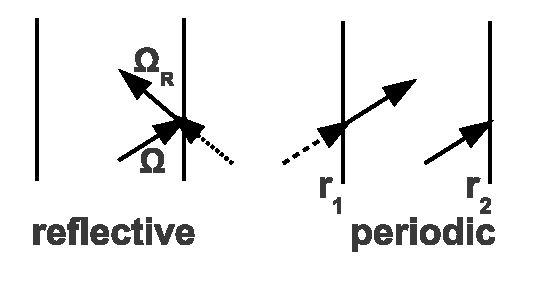
\includegraphics[keepaspectratio, width = 2.0 in]{images/reflectiveperiodic}
    \caption{Reflective and periodic boundary conditions.}
    \label{fig:reflectiveperiodic}
\end{figure}

The final boundary condition we mention is the \textit{white boundary condition}, a condition where all neutrons incident on a boundary reflect back isotropically in angle.  For this case,
\begin{equation}
\begin{split}
 \psi(\mathbf{r}_s,\mathbf{\Omega},E,t) &= \frac{ \int_{\mathbf{\hat{n}} \cdot \mathbf{\Omega}' > 0}   \mathbf{\hat{n}} \cdot \mathbf{\Omega}' \psi (\mathbf{r},\mathbf{\Omega}',E,t)d\Omega' } {  \int_{\mathbf{\hat{n}} \cdot \mathbf{\Omega}' > 0}  \mathbf{\hat{n}} \cdot \mathbf{\Omega}'  d\Omega'    }  \\
             &= \frac{ J_+ (\mathbf{r}_s,E,t) } {  \int_{\mathbf{\hat{n}} \cdot \mathbf{\Omega}' > 0}  \mathbf{\hat{n}} \cdot \mathbf{\Omega}'  d\Omega'    }\, , \, \, \, \,  \, \, \, \mathbf{\hat{n}} \cdot \mathbf{\Omega}' < 0 \, .
\end{split}
\end{equation}
Note the conditions on $\mathbf{\Omega}$ and $\mathbf{\Omega}'$.  The first corresponds to the left hand side and is limited to $\mathbf{\hat{n}} \cdot \mathbf{\Omega}' < 0$, i.e. incoming directions.  Contrarily, $\mathbf{\Omega}'$ is the dummy variable on the right hand side, and is always integrated over the domain where $\mathbf{\hat{n}} \cdot \mathbf{\Omega}' > 0$, i.e. outgoing directions.  This is so because we integrate the entire outgoing neutron population (which is proportional to the outgoing partial current) and then redistribute that number uniformly over all incident directions, i.e. isotropically.

White boundary conditions have had use in lattice physics where an isotropic angular distribution is sometimes relatively accurate.  In particular, the white boundary condition provides a useful fix for reflective conditions in Wigner-Seitz cells, which convert square pin cells into equivalent cylindrical cells, since cylindrical cells can be treated with 1-d methods.  However, while in square cells the reflective conditions work fine, they do not work well in cylindrical geometries (see Figure \ref{fig:wignerseitz}), since neutrons entering at certain angles can spend too much time in the moderator before colliding.  This consequently leads to overprediction of the moderator flux, an artifact known as the Newmarch effect. As a result, white conditions are used.


\begin{figure}[h] 
    \centering
    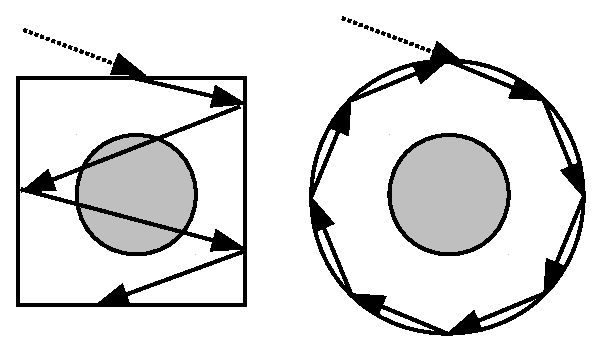
\includegraphics[keepaspectratio, width = 3.0 in]{images/wignerseitz}
    \caption{Square pin cell and equivalent Wigner-Seitz cell.  Same incident direction and location.}
    \label{fig:wignerseitz}
\end{figure}

\section*{Other Transport Equations}

We finish this lecture by presenting in brief two other important transport equations.

\subsection*{Photon Transport}

Photon transport is fundamental to radiation hydrodynamics (an integral aspect of ``bomb'' physics) and astrophysics.  Photon transport can largely be divided into two classes of problems: \textit{radiative transfer}, which consists of the propogation of soft (low energy) x-rays, and \textit{high energy} photon transport, which can largely be treated as we do neutrons.  We briefly describe the former.

The quantity of interest is the intensity, essentially an ``energy angular flux'', and is defined
\begin{equation}
 I_{\nu}(\mathbf{r},\mathbf{\Omega},t) = (h\nu)cn(\mathbf{r},\mathbf{\Omega},E,t) \, ,
\end{equation}
where $h\nu$ is the photon energy.  The ``radiative transfer equation'' is
\begin{equation}
 \frac{1}{c}\frac{\partial I_{\nu}}{\partial t} + \Omega \cdot \nabla I_{\nu} = \rho(\varepsilon_{\nu} - \kappa_{\nu}I_{\nu}) \, ,
 \label{eq:radiative}
\end{equation}
where $\varepsilon$ is a mass emission coefficient (a source term), and $\kappa$ is a mass attenuation coefficient (a loss term).  The radiative transfer equations are nonlinear due to the temperature-dependence of the underlying interaction coefficients (the ``cross-sections), particularly the emission term (which is not explicitly represented in Eq. \ref{eq:radiative}).

For the case of local thermodynamic equilibrium (LTE), Eq. \ref{eq:radiative} is simplified somewhat.  Local thermodynamic equilibrium exists when the quantity $S_{\nu} = \varepsilon_{\nu}/\kappa_{\nu} = B_{\nu}$, where $B_{\nu}$ is the Planck distribution (i.e. the black body spectrum).  In this case, Eq. \ref{eq:radiative} takes the form
\begin{equation}
 \frac{1}{c}\frac{\partial I_{\nu}}{\partial t} + \Omega \cdot \nabla I_{\nu} = \rho \kappa_{\nu} (B_{\nu} - I_{\nu}) \, .
 \label{eq:radiativelte}
\end{equation}

Radiative transfer is inherently a frequency-dependent process: the coefficients depend on the frequency, and a medium emits photons of a wide range of frequencies.  A frequently used approximation is to neglect this dependence in what is called the \textit{grey approximation}, similar to the one-speed studies in neutron transport we will study in the next several lectures.  ``Black bodies'' are also often used; these are pure absorbers whose emission spectrum is the Planck distribution.

To determine the temperature (dependence on which is implicit in all the quantities of Eq. \ref{eq:radiative}), an energy conservation equation is used.  As an example, using the grey approximation and assuming temperature- and spatially-independent coefficients, Eq. \ref{eq:radiative} becomes
\begin{equation}
 \frac{1}{c}\frac{\partial I}{\partial t} + \Omega \cdot \nabla I(\mathbf{r},\mathbf{\Omega},t) = \rho \kappa (acT^4(\mathbf{r},t)- I) \, ,
 \label{eq:radiativegrey}
\end{equation}
where $a$ is the emissivity (as in the Stefan-Boltzmann law) and $T$ is the temperature.  The corresponding energy conservation equation is
\begin{equation}
 \overbrace{c_v \frac{\partial T}{\partial t}}^{\text{energy rate of change}} = \overbrace{\rho \kappa}^{\text{abs. coef.}} \overbrace{\int_{4\pi} I(\mathbf{r},\mathbf{\Omega},t) d\Omega}^{\text{energy flux}} - \overbrace{\rho \kappa a c T^4(\mathbf{r},t)}^{\text{loss due to emission}} + \overbrace{Q(\mathbf{r},t)}^{\text{gains from outside}} \, ,
\end{equation}
where $c_v$ is the specific heat and $Q$ represents any external energy source.


\subsection*{Plasma Transport}

Another area of interest for nuclear engineers is plasma physics.  Let us apply Eq. \ref{eq:generalte} to electrons in a plasma, where we substitute in the Lorentz force for $\mathbf{F}$:
\begin{equation}
  \frac{\partial n}{\partial t} 
   + \mathbf{v} \cdot \nabla n + \frac{e}{m} \Big ( \mathbf{E}+(\mathbf{v}\times \mathbf{B} ) \Big ) \cdot \nabla_{\mathbf{v}} n =   \Big( \frac{\partial n}{\partial t} \Big )_{\mathrm{coll}} +  s \, .
\end{equation}
If we neglect sources and collisions, we arrive at the Vlasov equation:
\begin{equation}
  \frac{\partial n}{\partial t} 
   + \mathbf{v} \cdot \nabla n + \frac{e}{m} \Big ( \mathbf{E}+(\mathbf{v}\times \mathbf{B} ) \Big ) \cdot \nabla_{\mathbf{v}} n =  0 \, .
\end{equation}
Augmented with Maxwell's equations, the Vlasov equation gives a rather complete description of collisionless plasmas.  



\section*{Further Reading}
This lecture follows quite closely the treatment of transport theory in Chapter 1 of Duderstadt and Martin \cite{duderstadt1976tt}.  The reader is encouraged to read that chapter (uploaded to Stellar) and others (MIT libraries should have a copy for the eager beaver).  Bell and Glasstone \cite{bell1970nrt} give a more traditional derivation, as do Duderstadt and Hamilton \cite{duderstadt1976nra}.
 
The treatment of boundary conditions is rather straightforward, but the student may wish to consult e.g. Duderstadt and Martin \cite{duderstadt1976tt} or Lewis and Miller \cite{lewis1993cmn}.  The discussion of white boundary conditions and the Wigner-Seitz dilemma follows that of H\'{e}bert \cite{hebert2009arp}, and the Newmarch effect is identified by Stamm'ler and Abbate \cite{stammler1983mss}.   

The discussion of photon and plasma transport largely follows that of Duderstadt and Martin \cite{duderstadt1976tt}.  The example grey approximation equations are given in a paper by Miller and Lewis \cite{miller1987nrm}, and there is a wealth of literature on the subject.  For those interested in radiative transfer as it applies to atmospheres, see MIT course 12.815.

\begin{exercises}
 
  \item \textbf{Variable Transformations}. 
        Prove the relations given in Eq. \ref{eq:densityrelations}.

%   \item In Lecture \ref{lec:criticality}, the eigenvalue problem, i.e. a problem without an external source, was introduced in operator form.  You probably also know the eigenvalue diffusion equation from reactor physics. 
%   \begin{enumerate}[(a)]
%    \item Write down the 1-d, one group transport equation for an eigenvalue problem in slab geometry (you need to determine the fission source term)
%    \item Assuming isotropic scattering, and an infinite homogeneous, derive a simple expression for $k$ in terms of the cross-sections; what does this expression represent?
%   \end{enumerate}

  \item \textbf{Duderstadt \& Hamilton 4-3}. Suppose that the angular neutron 
        density is given by 
        \begin{equation*}
          n(\mathbf{r},\hat{\bm{\Omega}}) = \frac{n_0}{4\pi} (1-\cos\theta) \, ,
        \end{equation*}
        where $\theta$ is the angle between $\hat{\bm{\Omega}}$ and the 
        $z$-axis. If $A$ is the area perpendicular to the $z$-axis, then 
        what is the number of neutrons passing through the area 
        per second
        \begin{enumerate}[(a)]
         \item per unit solid angle at an angle of 45$^{\text{o}}$ with 
               the $z$-axis
         \item from the negative $z$ to the positive $z$ direction
         \item net 
         \item total?
        \end{enumerate}

  \item \textbf{Duderstadt \& Hamilton 4-4}. In a spherical thermal reactor of 
        radius $R$, it is found that the angular flux can be roughly 
        described by 
        \begin{equation*}
         \psi(\mathbf{r}, E, \hat{\bm{\Omega}}) 
          = \frac{\phi_0}{4\pi} E \exp \left ( -\frac{E}{kT} \right ) \frac{\sin(\pi r/R)}{r} \, .
        \end{equation*}
        Compute the total number of neutrons in the core.

  \item \textbf{Duderstadt \& Hamilton 4-5}. Demonstrate that in an 
        isotropic flux, the partial current density in any direction is
        given by $J_+ = \phi / 4$.


\end{exercises}

\chapter[Boundary Conditions]{Boundary and Initial Conditions, and Some Other Transport Equations}

The last lecture introduced both general transport equations and the neutron transport equation.  In this lecture, we discuss several boundary and interface conditions for constraining the transport equation.  We finish by briefly describing two additional transport equations that help us recognize special features of the neutron transport equation.

\section*{Boundary and Initial Condtions}

In the last lacture, we finished with the Eq. \ref{eq:neutrontransport} neutron transport equation:
\begin{equation*}
  \begin{split}
     \frac{1}{v}\frac{\partial \psi}{\partial t} &+ \hat{\Omega} \cdot \nabla \psi + \Sigma_t \psi(\mathbf{r},\mathbf{\Omega},E,t) = \\
           &+ \int^{\infty}_{0} dE' \int_{4\pi} d\Omega' \Sigma_s(\mathbf{r},\mathbf{\Omega}\cdot\mathbf{\Omega}',E'\to E)\psi(\mathbf{r},\mathbf{\Omega'},E',t) +s \, .
  \end{split}
\end{equation*}
This is an integro-differential equation in 7 variables: 3 in space, 2 in angle, 1 in energy, and time.  Like all differential equations, the transport equation requires initial and boundary conditions. 

\subsection*{Initial Conditions}

Initial conditions for the transport equation are relatively straightforward.  At some initial time $t_0$, an initial condition is expressed as
\begin{equation}
 \psi(\mathbf{r},\mathbf{\Omega},E,t)|_{t=t_0} = f(\mathbf{r},\mathbf{\Omega},E) \, ,
\end{equation}
where $f$ represents a known function of space, angle, and energy.  

Time-dependent problems in neutron transport are often quite challenging due to the wide range of time scales involved.  A good example comes from the study of reactor kinetics, where the time scales range from prompt neutron lifetimes (on the order of 10$^{-5}$ seconds) to the delayed neutrons of longest lifetime (on the order of tens of seconds).  Any numerical scheme is effectively limited by the smallest time scale, leading to a ``stiff'' problem.  

Other neutron transport problems exhibit even more diverse time scales.  The time scale for nuclear weapons is perhaps most easily quantified with ``shakes'', that is 10$^{-8}$ seconds.  Isotopic changes in nuclear reactors due to irradiation can have profound effects on time scales ranging from hours (xenon production) up to months or years (burnup).

Frequently, we are interested in steady state values, so that $\frac{\partial \psi}{\partial t} = 0$.  If the source $s$ in Eq. \ref{eq:neutrontransport} includes an external source, then the problem is a \textit{fixed source problem}.  If $s$ does not include an external source (and includes only e.g. a fission source), then the problem becomes an \textit{eigenvalue problem}, which are studied in Lecture \ref{lec:criticality}.

\subsection*{Boundary Conditions}

The most straightforward boundary condition to enforce is the \textit{free surface} or \textit{vacuum} condition.  Physically, the condition represents the situation where no neutrons enter a volume from the outside.  In other words, the volume of interest can be thought to exist in a void.  Mathematically, the condition is expressed
\begin{equation}
 \psi(\mathbf{r},\mathbf{\Omega},E,t) = 0 \, , \, \, \, \,  \, \, \, \mathbf{\hat{n}} \cdot \mathbf{\Omega} < 0 \, ,
\end{equation}
where $\mathbf{\hat{n}}$ is the unit \textit{outward normal} vector to the surface of interest.  
% is there a better way to give nice wrapping??  
\begin{wrapfigure}{r}{0.3\textwidth}
    \begin{center}
    \includegraphics[keepaspectratio, width = 1.25 in]{images/squarecylinder}
    \end{center}
    \caption{A reentrant square cyclinder.}
    \label{fig:squarecylinder}
\end{wrapfigure}
Since $\mathbf{\hat{n}} \cdot \mathbf{\Omega}$ is just the cosine of the angle between the incident neutrons and the normal vector, we see the flux vanishes whenever that cosine is negative, or whenever the neutron direction is inward.

A point of warning: reentrant geometries must be avoided when using vacuum conditions.  Unless treated with special care, reentrant geometries lead to inconsistency.  Neutrons leaving one portion of the geometry could, in theory, reenter another portion, but since vacuum conditions disallow this, the true problem is not modeled correctly.  A common example of this occurs when ``squaring'' an exterior cylindrical boundary, as exhibited in Figure \ref{fig:squarecylinder}.

Another useful boundary condition is simply to specify the incident flux when it is known:
\begin{equation}
 \psi(\mathbf{r}_s,\mathbf{\Omega},E,t) = f(\mathbf{r}_s,\mathbf{\Omega},E,t) \, .
\end{equation}
In this way, boundary sources can be defined.

A \textit{reflective} or \textit{specular} condition is such that 
\begin{equation}
 \psi(\mathbf{r}_s,\mathbf{\Omega},E,t) = \psi(\mathbf{r}_s,\mathbf{\Omega}_R,E,t) \, , \, \, \, \,  \, \, \, \mathbf{\hat{n}} \cdot \mathbf{\Omega} < 0 \, ,
\end{equation}
where $\mathbf{\Omega}_R$ is the (mirror) reflection of $\mathbf{\Omega}$.  Reflective conditions are widely used in lattice physics, where pin cells or assemblies are modeled in an infinite array; the ``infinite'' is captured by the reflective conditions.  See Figure \ref{fig:reflectiveperiodic}.

A variation on reflective conditions is an \textit{albedo} condition, where
\begin{equation}
 \psi(\mathbf{r}_s,\mathbf{\Omega},E,t) = \alpha \psi(\mathbf{r}_s,\mathbf{\Omega}_R,E,t) \, , \, \, \, \,  \, \, \, \mathbf{\hat{n}} \cdot \mathbf{\Omega} < 0 \, .
\end{equation}
Here, $\alpha$ is the ``albedo'' and quantifies the strength with which neutrons stream back into the system after streaming out.  Historically, albedo conditions were highly useful since they can often capture the physics of reflectors with minimum computational cost.  The albedos for many materials were precomputed (or found experimentally), effectively eliminating a significant portion of phase space in e.g. reactor analysis.

Another approach is to use \textit{periodic} conditions, such that
\begin{equation}
 \psi(\mathbf{r}_1,\mathbf{\Omega},E,t) = \psi(\mathbf{r}_2,\mathbf{\Omega},E,t) \, ,
\end{equation}
Figure \ref{fig:reflectiveperiodic} illustrates both reflective and periodic boundary conditions.  Periodic conditions work well in infinite arrays that have assymetric unit cells (for which reflective conditions would represent an infinite but incorrect array).

\begin{figure}[h] 
    \centering
    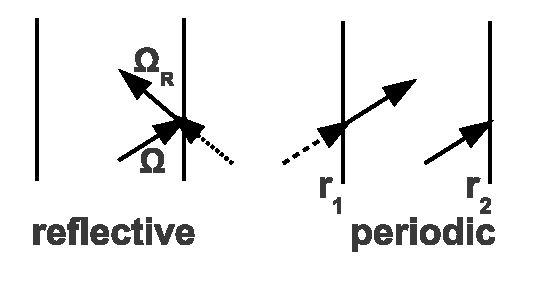
\includegraphics[keepaspectratio, width = 2.0 in]{images/reflectiveperiodic}
    \caption{Reflective and periodic boundary conditions.}
    \label{fig:reflectiveperiodic}
\end{figure}

The final boundary condition we mention is the \textit{white boundary condition}, a condition where all neutrons incident on a boundary reflect back isotropically in angle.  For this case,
\begin{equation}
\begin{split}
 \psi(\mathbf{r}_s,\mathbf{\Omega},E,t) &= \frac{ \int_{\mathbf{\hat{n}} \cdot \mathbf{\Omega}' > 0}   \mathbf{\hat{n}} \cdot \mathbf{\Omega}' \psi (\mathbf{r},\mathbf{\Omega}',E,t)d\Omega' } {  \int_{\mathbf{\hat{n}} \cdot \mathbf{\Omega}' > 0}  \mathbf{\hat{n}} \cdot \mathbf{\Omega}'  d\Omega'    }  \\
             &= \frac{ J_+ (\mathbf{r}_s,E,t) } {  \int_{\mathbf{\hat{n}} \cdot \mathbf{\Omega}' > 0}  \mathbf{\hat{n}} \cdot \mathbf{\Omega}'  d\Omega'    }\, , \, \, \, \,  \, \, \, \mathbf{\hat{n}} \cdot \mathbf{\Omega}' < 0 \, .
\end{split}
\end{equation}
Note the conditions on $\mathbf{\Omega}$ and $\mathbf{\Omega}'$.  The first corresponds to the left hand side and is limited to $\mathbf{\hat{n}} \cdot \mathbf{\Omega}' < 0$, i.e. incoming directions.  Contrarily, $\mathbf{\Omega}'$ is the dummy variable on the right hand side, and is always integrated over the domain where $\mathbf{\hat{n}} \cdot \mathbf{\Omega}' > 0$, i.e. outgoing directions.  This is so because we integrate the entire outgoing neutron population (which is proportional to the outgoing partial current) and then redistribute that number uniformly over all incident directions, i.e. isotropically.

White boundary conditions have had use in lattice physics where an isotropic angular distribution is sometimes relatively accurate.  In particular, the white boundary condition provides a useful fix for reflective conditions in Wigner-Seitz cells, which convert square pin cells into equivalent cylindrical cells, since cylindrical cells can be treated with 1-d methods.  However, while in square cells the reflective conditions work fine, they do not work well in cylindrical geometries (see Figure \ref{fig:wignerseitz}), since neutrons entering at certain angles can spend too much time in the moderator before colliding.  This consequently leads to overprediction of the moderator flux, an artifact known as the Newmarch effect. As a result, white conditions are used.


\begin{figure}[h] 
    \centering
    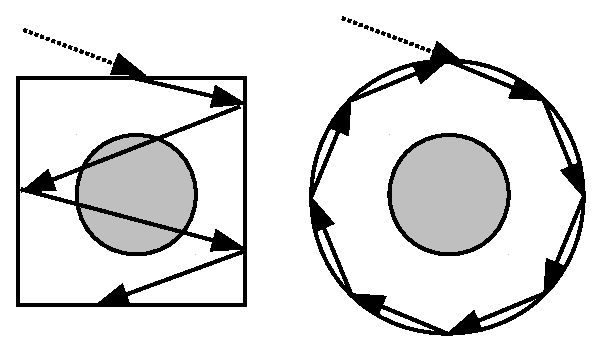
\includegraphics[keepaspectratio, width = 3.0 in]{images/wignerseitz}
    \caption{Square pin cell and equivalent Wigner-Seitz cell.  Same incident direction and location.}
    \label{fig:wignerseitz}
\end{figure}

\section*{Other Transport Equations}

We finish this lecture by presenting in brief two other important transport equations.

\subsection*{Photon Transport}

Photon transport is fundamental to radiation hydrodynamics (an integral aspect of ``bomb'' physics) and astrophysics.  Photon transport can largely be divided into two classes of problems: \textit{radiative transfer}, which consists of the propogation of soft (low energy) x-rays, and \textit{high energy} photon transport, which can largely be treated as we do neutrons.  We briefly describe the former.

The quantity of interest is the intensity, essentially an ``energy angular flux'', and is defined
\begin{equation}
 I_{\nu}(\mathbf{r},\mathbf{\Omega},t) = (h\nu)cn(\mathbf{r},\mathbf{\Omega},E,t) \, ,
\end{equation}
where $h\nu$ is the photon energy.  The ``radiative transfer equation'' is
\begin{equation}
 \frac{1}{c}\frac{\partial I_{\nu}}{\partial t} + \Omega \cdot \nabla I_{\nu} = \rho(\varepsilon_{\nu} - \kappa_{\nu}I_{\nu}) \, ,
 \label{eq:radiative}
\end{equation}
where $\varepsilon$ is a mass emission coefficient (a source term), and $\kappa$ is a mass attenuation coefficient (a loss term).  The radiative transfer equations are nonlinear due to the temperature-dependence of the underlying interaction coefficients (the ``cross-sections), particularly the emission term (which is not explicitly represented in Eq. \ref{eq:radiative}).

For the case of local thermodynamic equilibrium (LTE), Eq. \ref{eq:radiative} is simplified somewhat.  Local thermodynamic equilibrium exists when the quantity $S_{\nu} = \varepsilon_{\nu}/\kappa_{\nu} = B_{\nu}$, where $B_{\nu}$ is the Planck distribution (i.e. the black body spectrum).  In this case, Eq. \ref{eq:radiative} takes the form
\begin{equation}
 \frac{1}{c}\frac{\partial I_{\nu}}{\partial t} + \Omega \cdot \nabla I_{\nu} = \rho \kappa_{\nu} (B_{\nu} - I_{\nu}) \, .
 \label{eq:radiativelte}
\end{equation}

Radiative transfer is inherently a frequency-dependent process: the coefficients depend on the frequency, and a medium emits photons of a wide range of frequencies.  A frequently used approximation is to neglect this dependence in what is called the \textit{grey approximation}, similar to the one-speed studies in neutron transport we will study in the next several lectures.  ``Black bodies'' are also often used; these are pure absorbers whose emission spectrum is the Planck distribution.

To determine the temperature (dependence on which is implicit in all the quantities of Eq. \ref{eq:radiative}), an energy conservation equation is used.  As an example, using the grey approximation and assuming temperature- and spatially-independent coefficients, Eq. \ref{eq:radiative} becomes
\begin{equation}
 \frac{1}{c}\frac{\partial I}{\partial t} + \Omega \cdot \nabla I(\mathbf{r},\mathbf{\Omega},t) = \rho \kappa (acT^4(\mathbf{r},t)- I) \, ,
 \label{eq:radiativegrey}
\end{equation}
where $a$ is the emissivity (as in the Stefan-Boltzmann law) and $T$ is the temperature.  The corresponding energy conservation equation is
\begin{equation}
 \overbrace{c_v \frac{\partial T}{\partial t}}^{\text{energy rate of change}} = \overbrace{\rho \kappa}^{\text{abs. coef.}} \overbrace{\int_{4\pi} I(\mathbf{r},\mathbf{\Omega},t) d\Omega}^{\text{energy flux}} - \overbrace{\rho \kappa a c T^4(\mathbf{r},t)}^{\text{loss due to emission}} + \overbrace{Q(\mathbf{r},t)}^{\text{gains from outside}} \, ,
\end{equation}
where $c_v$ is the specific heat and $Q$ represents any external energy source.


\subsection*{Plasma Transport}

Another area of interest for nuclear engineers is plasma physics.  Let us apply Eq. \ref{eq:generalte} to electrons in a plasma, where we substitute in the Lorentz force for $\mathbf{F}$:
\begin{equation}
  \frac{\partial n}{\partial t} 
   + \mathbf{v} \cdot \nabla n + \frac{e}{m} \Big ( \mathbf{E}+(\mathbf{v}\times \mathbf{B} ) \Big ) \cdot \nabla_{\mathbf{v}} n =   \Big( \frac{\partial n}{\partial t} \Big )_{\mathrm{coll}} +  s \, .
\end{equation}
If we neglect sources and collisions, we arrive at the Vlasov equation:
\begin{equation}
  \frac{\partial n}{\partial t} 
   + \mathbf{v} \cdot \nabla n + \frac{e}{m} \Big ( \mathbf{E}+(\mathbf{v}\times \mathbf{B} ) \Big ) \cdot \nabla_{\mathbf{v}} n =  0 \, .
\end{equation}
Augmented with Maxwell's equations, the Vlasov equation gives a rather complete description of collisionless plasmas.  

\section*{Further Reading}

The treatment of boundary conditions is rather straightforward, but the student may wish to consult e.g. Duderstadt and Martin \cite{duderstadt1976tt} or Lewis and Miller \cite{lewis1993cmn}.  The discussion of white boundary conditions and the Wigner-Seitz dilemma follows that of H\'{e}bert \cite{hebert2009arp}, and the Newmarch effect is identified by Stamm'ler and Abbate \cite{stammler1983mss}.   

The discussion of photon and plasma transport largely follows that of Duderstadt and Martin \cite{duderstadt1976tt}.  The example grey approximation equations are given in a paper by Miller and Lewis \cite{miller1987nrm}, and there is a wealth of literature on the subject.  For those interested in radiative transfer as it applies to atmospheres, see MIT course 12.815.




\include{analytical_solutions}
\chapter{The Integral Form}

In this lecture we consider the integral form of the transport equation in both general coordinates and the specific case of slab geometry.  The integral form is useful in situations where only the scalar flux is required and is the foundation for the collision probabability method, which we cover in the next lecture, as well as the method of characteristics, fast becoming the technique of choice in reactor analysis.  We consider some analytical aspects of the integral equation and finish by discussing a simple numerical approach based on Von Neumann series expansions.

\section*{The Integral Transport Equation}

You may have noticed from the previous two lectures that the angular dependence of the particle density is a relatively unique aspect of transport processes.  Often, this angular dependence is the hardest aspect that we deal with directly, either analytically or numerically\footnote{Energy is by far more complex, as we've noted, and there are very few analytical problems where energy can be handled directly (slowing down in an infinite homogeneous medium problem is one example). Consequently, we typically use only the crudest representation possible in discretizing the energy variable, though much physics goes into generating the discrete data.}  It would be nice to eliminate the angular variable completely, and for certain problems, the \textit{ integral transport equation} allows us to do with a minimum of approximation.

Before we derive the integral form of the transport equation, it helps define a new quantity called the \textit{emission density},
\begin{equation}
  Q(\mathbf{r},\mathbf{\Omega}) = \int_{4\pi} d\Omega' \Sigma_s(\mathbf{r},\mathbf{\Omega}\cdot\mathbf{\Omega}')\psi(\mathbf{r},\mathbf{\Omega'}) + S(\mathbf{r},\mathbf{\Omega}) \, .
  \label{eq:emissiondensity}
\end{equation}
Essentially, $Q$ is a generalized source containing any external source $S$ and scattering source; of course, fission could also be included.

Recall the discussion of Eq. \ref{eq:spaceratepsi}, where we consider a distance $s$ from some reference point $\mathbf{r}_0$ along the characteristic $\mathbf{r}_0 +s\mathbf{\Omega}$.  The full transport equation in terms of $s$ is 
\begin{equation}
    \frac{d}{ds} \psi(\mathbf{r}_0 +s\mathbf{\Omega},\mathbf{\Omega}) + \Sigma_t(\mathbf{r}_0 +s\mathbf{\Omega})\psi =   Q(\mathbf{r}_0 +s\mathbf{\Omega},\mathbf{\Omega})  \, ,
    \label{eq:forchareq}
\end{equation}
which can be called the \textit{forward characteristic} equation, as we follow neutrons forward from the reference point.  Similar, and which we use below, is the \textit{backward characteristic} form, which represents following neutrons backward along the characteristic from a current point $\mathbf{r}$.  Let $p = -s$.  Then $d/dp = -d/ds$ and Eq. \ref{eq:forchareq} becomes (after dropping the $0$ subscript from $\mathbf{r}$)
\begin{equation}
    -\frac{d}{dp} \psi(\mathbf{r} - p\mathbf{\Omega},\mathbf{\Omega}) + \Sigma_t(\mathbf{r} -p\mathbf{\Omega})\psi =   Q(\mathbf{r} -p\mathbf{\Omega},\mathbf{\Omega})  \, .
    \label{eq:backchareq}
\end{equation}
We wish to integrate from $p=0$ to some maximum distance (eventually to be either infinity or a global boundary).  Introducing the integrating factor
\begin{equation}
 if = e^{ -\int^p_0 \Sigma_t(\mathbf{r} -p'\mathbf{\Omega}) dp'  } \, 
\end{equation}
into Eq. \ref{eq:backchareq}, we have
\begin{equation}
    -\frac{d}{dp} \Big ( \psi(\mathbf{r}_0 - p\mathbf{\Omega},\mathbf{\Omega}) e^{ -\int^p_0 \Sigma_t(\mathbf{r} -p'\mathbf{\Omega}) dp'  } \Big ) =  Q(\mathbf{r} -p\mathbf{\Omega}) e^{ -\int^p_0 \Sigma_t(\mathbf{r} -p'\mathbf{\Omega}) dp'  } \, ,
\end{equation}
and integrating
\begin{equation}
  \begin{split}
    -\int^{\psi(p'=p)}_{\psi(p=0)}  \Bigg(  d \Big ( \psi(\mathbf{r} &- p'\mathbf{\Omega},\mathbf{\Omega})   e^{ -\int^{p'}_0 \Sigma_t(\mathbf{r} -p''\mathbf{\Omega}) dp''  } \Big ) \Bigg ) = \\
   & \int^p_0 Q(\mathbf{r} -p'\mathbf{\Omega},\mathbf{\Omega})e^{ -\int^{p'}_0 \Sigma_t(\mathbf{r} -p''\mathbf{\Omega}) dp''  }dp'   \\
  \end{split}
\end{equation}
yields
\begin{equation}
  \begin{split}
    \psi(\mathbf{r},\mathbf{\Omega}) - \psi(\mathbf{r} &- p\mathbf{\Omega},\mathbf{\Omega})e^{ -\int^{p}_0 \Sigma_t(\mathbf{r} -p''\mathbf{\Omega}) dp''  }  = \\
   & \int^p_0 Q(\mathbf{r} -p'\mathbf{\Omega},\mathbf{\Omega})e^{ -\int^{p'}_0 \Sigma_t(\mathbf{r} -p''\mathbf{\Omega}) dp''  }dp'   \, .
  \end{split}
\end{equation}

We can simplify the notation somewhat by defining the \textit{optical pathlength} $\tau$, such that
\begin{equation}
  \tau ( \mathbf{r} ,\mathbf{r} -p \mathbf{\Omega} ) = \int^p_0 \Sigma_t(\mathbf{r} -p'\mathbf{\Omega}) dp' \, . 
  \label{eq:opticalpathlength}
\end{equation}
Then, the integral equation for the angular flux becomes
\begin{equation}
  \begin{split}
    \psi(\mathbf{r},\mathbf{\Omega}) = \int^p_0 Q(\mathbf{r} -p'\mathbf{\Omega},\mathbf{\Omega})e^{-\tau(\mathbf{r},\mathbf{r}-p'\mathbf{\Omega})}dp'                         +  \psi(\mathbf{r} - p\mathbf{\Omega},\mathbf{\Omega})e^{ -\tau(\mathbf{r},\mathbf{r}-p\mathbf{\Omega}) }   \, .
  \end{split}
  \label{eq:inteqpsi}
\end{equation}

In many cases, the emission density $Q$ is assumed to be isotropic in the lab system.  In this case, we can integrate out the angular dependence and arrive at an integral equation for the scalar flux often referred to as Peierl's equation.  To do so, we let the integration bound $p$ of Eq. \ref{eq:inteqpsi} go to infinity.  We assume the second term on the right hand side to vanish (i.e. either $\psi$ vanishes at infinity, or equivalently, the optical path length $\tau(\mathbf{r},\infty)$ goes to $\infty$, and so the exponential vanishes).  

Letting $Q(\mathbf{r},\mathbf{\Omega}) = Q(\mathbf{r} -p\mathbf{\Omega})/4\pi$, and substituting $\mathbf{r}' = \mathbf{r} - p \mathbf{\Omega}$, we integrate Eq. \ref{eq:inteqpsi} over all angles to get
\begin{equation}
 \phi(\mathbf{r}) = \int_{4\pi} d\Omega \int^{\infty}_0  \frac{Q(\mathbf{r}')}{4\pi}e^{-\tau(\mathbf{r},\mathbf{r}')}dp \, .
 \label{eq:integralphiPRE}
\end{equation}
Now note that $p =|\mathbf{\Omega} p|=|\mathbf{r}-\mathbf{r}'|$, and consequently $p^2 = |\mathbf{r}-\mathbf{r}'|^2$.  Multiplying within the integrand by $1=p^2/|\mathbf{r}-\mathbf{r}'|^2$ yields
\begin{equation}
 \phi(\mathbf{r}) = \int_{4\pi} d\Omega \int^{\infty}_0  \frac{Q(\mathbf{r}')}{4\pi}e^{-\tau(\mathbf{r},\mathbf{r}')}\frac{p^2dp}{|\mathbf{r}-\mathbf{r}'|^2} \, ,
\end{equation}
and if the reader thinks this looks suspiciously like a volume integral in spherical coordinates, she would be right.  Letting $dV' = 4\pi d\Omega dpp^2$, we have
\begin{equation}
 \phi(\mathbf{r}) = \int_{V'} \frac{ Q(\mathbf{r}')e^{-\tau(\mathbf{r},\mathbf{r}')} dV'}{4\pi|\mathbf{r}-\mathbf{r}'|^2} \, .
 \label{eq:integralphi}
\end{equation}

\section*{Integral Transport in Slab Geometry}

We now look at the special case of Eq. \ref{eq:integralphi} in slab geometry, for which the emission density is a function only of $x$, i.e. $Q(\mathbf{r}) = Q(x)$.  We make use of cylindrical coordinates, with the axis taken to be $x$.  Our goal will be to integrate out the radial ($\rho$) and azimuthal ($\omega$) spatial components, leaving just the $x$ dependence. The differential volume is then
\begin{equation}
 dV' = \rho d\rho d\omega dx' ,
\end{equation}
and Eq. \ref{eq:integralphi} becomes
\begin{equation}
\begin{split}
 \phi(x) &= \int^{\infty}_{-\infty} dx' \int^{\infty}_0 d\rho \rho \int^{2\pi}_0 \frac{ d\omega' Q(x')e^{-\tau(\mathbf{r},\mathbf{r}')}}{4\pi|\mathbf{r}-\mathbf{r}'|^2} \, \\
        &= 2\pi \int^{\infty}_{-\infty}dx' \int^{\infty}_0 d\rho \rho \frac{ Q(x')e^{-\tau(\mathbf{r},\mathbf{r}')}}{4\pi |\mathbf{r}-\mathbf{r}'|^2} \, .
\end{split}
\label{eq:integralphix}
\end{equation}

We now need to express $\mathbf{r}$ and $\rho$ in terms of $x$.  Since the cross-sections (as quantified by $\tau$) are really dependent only on $x$, we can relate the full distance $|\mathbf{r}' - \mathbf{r}|$ with its projection along the $x$ axis via a directional cosine $\lambda^{-1}$ such that
\begin{equation}
 \lambda = \frac{|\mathbf{r}' - \mathbf{r}|}{|x'-x|} \, 
 \label{eq:projection}
\end{equation}
and $\tau(\mathbf{r}',\mathbf{r}) = \lambda \tau(x',x)$.  Moreover,
\begin{equation}
 |\mathbf{r}' - \mathbf{r}|^2 = \rho^2 + |x' - x|^2 \, 
\end{equation}
which, using Eq. \ref{eq:projection}, can be rewritten as
\begin{equation}
 \rho^2 = (\lambda^2 -1 )|x'-x|^2 \, ,
\end{equation}
and differentiating, we find
\begin{equation}
 \rho d\rho = \lambda d\lambda |x'-x|^2 \, .
\end{equation}
Noting that $\rho = 0$ corresponds to $\lambda = 1$, Eq. \ref{eq:integralphix} can be written in terms of $\lambda$ to give
\begin{equation}
\begin{split}
 \phi(x) &= 2\pi \int^{\infty}_{-\infty}dx' \int^{\infty}_1 \lambda d\lambda \frac{|x'-x|^2 }{4\pi|\mathbf{r}' - \mathbf{r}|^2}    Q(x')e^{-\tau(\mathbf{x},\mathbf{x}')} \\
        &= 2\pi \int^{\infty}_{-\infty}dx' \int^{\infty}_1 \lambda d\lambda \frac{1}{4\pi \lambda^2}    Q(x')e^{-\tau(\mathbf{x},\mathbf{x}')} \\       
        &=  \int^{\infty}_{-\infty} dx'\frac{1}{2} \int^{\infty}_1 \lambda d\lambda\frac{1}{\lambda}  Q(x')e^{-\tau(\mathbf{x},\mathbf{x}')} \, 
\end{split}
\end{equation}
or
\begin{equation}
 \phi(x) =  \int^{\infty}_{-\infty} dx'\frac{1}{2} E_1(\tau(\mathbf{x},\mathbf{x}'))Q(x') \, ,   
 \label{eq:integralphislab}     
\end{equation}
where we have used the $E_1$ function defined at the end of Lecture \ref{lec:analytical}.  

\section*{First-Flight Kernels}

Eq. \ref{eq:integralphislab} gives us an example of the use of a \textit{first-flight kernel} for the scalar flux, the general use of which takes the form
\begin{equation}
 \phi(\mathbf{r}) = \int d^3\mathbf{r}' k(\mathbf{r},\mathbf{r}')Q(\mathbf{r}') \, 
\end{equation}
for a kernel $k(\mathbf{r},\mathbf{r'})$.  For slab geometry, the first-flight kernel is seen to be
\begin{equation}
 k_{\text{slab}}(x,x') = \frac{1}{2} E_1(\tau(x,x')) \, .
 \label{eq:firstflightkernelslab}
\end{equation}

First-flight kernels have a particularly easy (and important!) physical interpretation. Consider Eq. \ref{eq:integralphislab} for the case of a purely absorbing medium.  Then the emissivity $Q$ consists only of external sources.  To help visualize the problem, take $Q$ to be a delta function at $x_0$, i.e. $Q(x) = Q_0 \delta(x-x_0)$.  Substituting this into Eq. \ref{eq:integralphislab} gives
\begin{equation}
 \phi(x) = \frac{1}{2} E_1(\tau(x,x_0)) Q_0 \, . 
\end{equation}
Thus, the kernel $k(x,x')$ can be seen to give the contribution of the source particles born at $x'$ to the flux at $x$.  In other words, it gives to us the \textit{uncollided flux}.  For many systems, having the uncollided flux can be a good approximation for the total flux, and in some numerical schemes, it can be a good initial guess to help reduce computational time and numerical artifacts (e.g. the discrete ordinates method, discussed in Lecture \ref{lec:discreteordinates}).

If we look back at the Peierl's equation (Eq. \ref{eq:integralphi}), we find the fundamental first-flight kernel of the point source, 
\begin{equation}
 k_{\text{point}}(\mathbf{r},\mathbf{r}') = \frac{e^{-\tau(\mathbf{r},\mathbf{r}')}}{4\pi|\mathbf{r}-\mathbf{r}'|^2} \, .
 \label{eq:firstflighkernelpoint}
\end{equation}

Two things are worth noting about Eq. \ref{eq:firstflighkernelpoint}.  First, the first-flight kernels for all other geometrical configurations can be derived from this kernel.  A second point, related to the first, is that the point kernel is closely related to the \textit{Green's function} for the transport equation.  

\section*{Green's Functions}


A Green's function $G(x,x')$ for a linear differential operator\footnote{We'll discuss the linearity of the transport equation in Lecture \ref{lec:linearity}, and we'll use operator notation extensively in Lecture \ref{lec:adjoint}.} $L=L(x)$ is defined
\begin{equation}
 LG(x,x') = \delta(x-x') \, .
 \label{eq:greens}
\end{equation}
A linear differential operator is any linear combination of basic differentiation operators.  $L$ could be $d/dx$ or $d^2/dx^2$ or $d^2/dx^2 + d/dx$, and so on.  The utility of $G$ arises when we wish to solve the inhomogeneous differential equation
\begin{equation}
 Lu(x) = f(x) \, .
 \label{eq:diffeq}
\end{equation}
If we multiply both sides of Eq. \ref{eq:greens} by $f(x')$ and integrate over $x'$, we find
\begin{equation}
 \int LG(x,x')f(x')dx' = \int dx' \delta(x-x') f(x') = f(x) \, ,
\end{equation}
but this suggests that
\begin{equation}
 Lu(x) = \int LG(x,x')f(x')dx' = L \int G(x,x')f(x')dx'  \, ,
\end{equation}
or 
\begin{equation}
 u(x) = \int G(x,x')f(x')dx'  \, .
\end{equation}
Hence, if we know $G(x,x')$, then we can solve the inhomogeneous equation for $u$.  

What about the transport equation?  Consider again Eq. \ref{eq:inteqpsi}, neglecting the second term, and letting $p\to \infty$, i.e. 
\begin{equation}
  \begin{split}
    \psi(\mathbf{r},\mathbf{\Omega}) = \int^{\infty}_0 Q(\mathbf{r} -p\mathbf{\Omega},\mathbf{\Omega})e^{-\tau(\mathbf{r},\mathbf{r}-p\mathbf{\Omega})}dp                          \, .
  \end{split}
  \label{eq:inteqpsi2}
\end{equation}
Note that this is still integrating along the characteristic.  It is more convenient to cast this as volume integral, similar to what we did above for Eq. \ref{eq:integralphi}.  However, even in volume form, we still want the integration confined to the characteristic.  By defining
\begin{equation}
 \delta(\mathbf{\Omega}\cdot\mathbf{\Omega}') \equiv \delta(\mu-\mu')\delta(\phi-\phi') \, ,
\end{equation}
and
\begin{equation}
 \mathbf{\Omega}_R \equiv \frac{\mathbf{r} -\mathbf{r}'}{|\mathbf{r}-\mathbf{r}'|} \, ,
\end{equation}
and recalling $p = |\mathbf{r}-\mathbf{r}'|$, we can rewrite Eq. \ref{eq:inteqpsi2} as
\begin{equation}
    \psi(\mathbf{r},\mathbf{\Omega}) = \int_{4\pi} d\Omega_R \delta(\mathbf{\Omega}\cdot\mathbf{\Omega}_R) \int^{\infty}_0 Q(\mathbf{r}',\mathbf{\Omega}_R)e^{-\tau(\mathbf{r},\mathbf{r'})}dp                          \, .
\end{equation}
Using $dV' = p^2dpd\Omega_R$, this becomes
\begin{equation}
    \psi(\mathbf{r},\mathbf{\Omega}) = \int_{V'} dV' \frac{1}{|\mathbf{r}-\mathbf{r}'|^2} \delta(\mathbf{\Omega}\cdot\mathbf{\Omega}_R)  Q(\mathbf{r}',\mathbf{\Omega}_R)e^{-\tau(\mathbf{r},\mathbf{r'})}                          \, .
\end{equation}

Now let $Q$ be a delta source at $\mathbf{r}_0$ emitting particles in direction $\mathbf{\Omega}_0$, or  $Q = \delta(\mathbf{r}-\mathbf{r}_0)\delta(\Omega\cdot\Omega_0)$, similar to the right hand side of Eq. \ref{eq:greens}. Then
\begin{equation}
  \begin{split}
    \psi(\mathbf{r},\mathbf{\Omega}) &= \int_{V'} dV' \frac{e^{-\tau(\mathbf{r},\mathbf{r'})} }{|\mathbf{r}-\mathbf{r}'|^2} \delta(\mathbf{\Omega}\cdot\mathbf{\Omega}_R) \delta(\mathbf{r}-\mathbf{r}_0)\delta(\mathbf{\Omega}\cdot\mathbf{\Omega}_0)                           \\
    &= \frac{e^{-\tau(\mathbf{r},\mathbf{r}_0)} }{|\mathbf{r}-\mathbf{r}_0|^2} \delta \Bigg (\mathbf{\Omega}\cdot \frac{\mathbf{r} -\mathbf{r}_0}{|\mathbf{r}-\mathbf{r}_0|} \Bigg ) \delta(\mathbf{\Omega}\cdot\mathbf{\Omega}_0) \\
    &= G_{\text{point}}(\mathbf{r},\mathbf{\Omega};\mathbf{r}_0,\mathbf{\Omega}_0) \, .
  \end{split}
  \label{eq:psigreen}
\end{equation}
This is the Green's function for the angular flux, with which we can find $\psi$ for any emission density $Q(\mathbf{r},\mathbf{\Omega}$)\footnote{Careful! If $Q$ includes scattering, then it depends on $\psi$, and so a direct solution in this form is not possible}.   We can use $G_{\text{point}}$ to recover the scalar flux point kernel by letting $Q$ be a unit isotropic point source, i.e. $Q = \delta(\mathbf{r}-\mathbf{r}_0)/4\pi$.  Then
\begin{equation}
\begin{split}
    \psi(\mathbf{r},\mathbf{\Omega}) &=  \int_V dV' \int_{4\pi} d\Omega' G_{\text{point}}(\mathbf{r},\mathbf{\Omega};\mathbf{r}',\mathbf{\Omega}') \frac{\delta(\mathbf{r}'-\mathbf{r}_0)}{4\pi} \\
    &= \frac{e^{-\tau(\mathbf{r},\mathbf{r}_0)} }{4\pi|\mathbf{r}-\mathbf{r}_0|^2} \delta \Bigg (\mathbf{\Omega}\cdot \frac{\mathbf{r} -\mathbf{r}_0}{|\mathbf{r}-\mathbf{r}_0|} \Bigg ) \, .
\end{split}
\label{eq:psiisosource}
\end{equation}
Integrating $\psi$ over all angles yields
\begin{equation}
\begin{split}
    \phi(\mathbf{r}) &=  \int_{4\pi} d\Omega \frac{e^{-\tau(\mathbf{r},\mathbf{r}_0)} }{4\pi|\mathbf{r}-\mathbf{r}_0|^2} \delta \Bigg (\mathbf{\Omega}\cdot \frac{\mathbf{r} -\mathbf{r}_0}{|\mathbf{r}-\mathbf{r}_0|} \Bigg ) \\
    &= \frac{e^{-\tau(\mathbf{r},\mathbf{r}_0)} }{4\pi|\mathbf{r}-\mathbf{r}_0|^2} \, ,
\end{split}
\end{equation}
which is indeed our point kernel for the scalar flux.

\section*{Neumann Series}

Lecture \ref{lec:cpm} will cover the widely-used collision probability method that is based on the integral transport equation.  Here, we investigate a less versatile yet quite enlightening method based on expansion of the scalar flux in a so-called Neumann\footnote{Carl Neumann, not to be confused with John von Neumann.} series for slab problems that include scattering.

Consider the integral equation in a slab of length $L$:
\begin{equation}
 \phi(x) = \int^L_0  dx' \frac{1}{2} E_1(\tau(x,x'))(S(x') + \phi(x')\Sigma_s(x')) \, .
\end{equation}
Defining the operator $K$,
\begin{equation}
 K\phi = \int^L_0  dx' \frac{1}{2} E_1(\tau(x,x'))\phi(x) \Sigma_s(x) \, ,
\end{equation}
we can rewrite the integral equation as
\begin{equation}
 (I-K)\phi = K\frac{S}{\Sigma_s} \, .
 \label{eq:integraloperatorform}
\end{equation}
Without going into formal detail (though it should seem ``reasonable''), Eq. \ref{eq:integraloperatorform} can be solved by expanding
\begin{equation}
 (I-K)^{-1} = I + K + K^2 + \ldots \, ,
\end{equation}
where $I$ is the identity operator, so that 
\begin{equation}
 \phi(x) = \sum^{\infty}_{n=0} K^n \frac{S(x)}{\Sigma_s(x)} \, .
 \label{eq:neumannseries}
\end{equation}

Suppose we define
\begin{equation}
 \phi_n(x) \equiv K^n \frac{S(x)}{\Sigma_s(x)} \, .
\end{equation}
Then we see that $\phi_0 = K(S/\Sigma_s)$, $\phi_1 = K^2(S/\Sigma_s) = K(\phi_0)$ and so on.  We recognize $\phi_0(x)$ as the uncollided flux, which is then used as input for $\phi_1$.  We recognize $\phi_1$ as those neutrons already having undergone a single collision (and no more).  In general, we call $\phi_n$ the $n$th collided flux.  The Neumann series Eq. \ref{eq:neumannseries} just adds up all neutrons that have not collided, those that have collided once, those that have twice, and so on, thus capturing the entire population of neutrons in the system.  Defining (and computing)  $\phi_n$ in terms of the previous term $\phi_{n-1}$ sequence is called \textit{Neumann iteration}.

\section*{A Numerical Example}

We illustrate the use of Neumann iteration in a simple MATLAB code for a homogeneous slab problem with a uniform isotropic source.  The integrals involved are approximated using the trapezoid rule, though the exercises explore other schemes.  Please refer to the code comments in Listing \ref{list:neumann_slab} to understand the exact implementation of the algorithm.


\lstset{language=Octave,caption=Solution of Slab Problem via Neumann Series, label=list:neumann_slab}
\lstinputlisting{code/neumann_slab.m}

\section*{Further Reading}

The derivation of the integral equations generally follow that of Lewis and Miller \cite{lewis1993cmn}.  First-flight kernels and Green's functions are covered in Duderstadt and Martin \cite{duderstadt1976tt} and Case and Zweifel \cite{case1967ltt}.  Solving for the scalar flux via Neumann iterations is discussed in Duderstadt and Martin \cite{duderstadt1976tt}, while its use as a general technique for integral equations is described e.g. by Arfken and Weber. Any good numerical analysis textbook will provide more information on numerical integration, and the reader is encouraged to explore this fundamental topic.    

\begin{exercises}
  
  \item \textbf{Point-to-slab}. Show how $k_{\text{slab}}$ can be generated using $k_{\text{point}}$.
  \item \textbf{Line source}. Show that the first-flight kernel for an infinite isotropic line source is given by
        \begin{equation}
         k_{\text{line}}(r,r') = \frac{1}{2\pi r}Ki_1(\Sigma_t|r-r'|) \, ,
         \label{eq:linekernel}
        \end{equation}
        where
        \begin{equation}
         Ki_n(x) = \int^{\pi/2}_0 \cos^{n-1}(\theta) e^{-x/\cos(\theta)}d\theta = \int^{\infty}_0 \frac{e^x \cosh(u)}{\cosh^n(u)} \, 
        \end{equation}
        are the Bickley-Naylor function of order $n$, and where $Ki_0(r) = K_0(r)$, the zeroth order modified Bessel function.

  \item \textbf{Spherical shell}. Show that the first-flight kernel for a spherical shell is given by
        \begin{equation}
         k_{\text{sph}}(r,r') = \frac{r'}{2r}Ki_1(\Sigma_t|r-r'|-\Sigma_t|r+r'|) \, ,
         \label{eq:sphericalkernel}
        \end{equation}

  \item \textbf{Current density kernels}. In the lecture found the flux kernel for a plane source, and the kernels for line and spherical sources are given in the first two exercises.  We can also derive kernels for the current density.  For example, in a slab, there is a current kernel $\gamma_{\text{slab}}(x,x')$ such that
  \begin{equation}
   \mathbf{J}(x) = \int^L_0 \gamma_{\text{slab}}(x,x') Q(x') dx' \, .
  \end{equation}
  Derive this kernel $\gamma_{\text{slab}}(x,x')$.
 
  \item \textbf{Using kernels}. Use $k_{\text{slab}}$ to find the scalar flux for the example of Lecture \ref{lec:analytical}, and use $\gamma_{\text{slab}}$ to find the corresponding current density.

  \item  \textbf{Von Neumann Series}. Use the Von Neumann series code for the slab in Listing \ref{list:neumann_slab} to plot the scalar flux, uncollided flux, and the first five collided fluxes on the same graph using 20 spatial divisions for $L = 10$, $\Sigma_t = 1.0$, and (a) $\Sigma_s = 0.2$ and (b) $\Sigma_s = 0.8$.  What changes for the case with higher scattering?

  \item \textbf{Convergence}. For the same problem, modify the Von Neumann series code to compute as many collided fluxes are necessary so that
  \begin{equation*}
   \frac{|\phi_n(x_i)-\phi_n(x_{i-1})|}{\phi_n(x_{i-1}} < \epsilon = 1\times10^{-6} \, \, \, \, \, \, \forall \, x_i \, ,
  \end{equation*}
   and comment on the results. (Hint, which norm on the $x$ vector is appropriate?)
  
  \item \textbf{Nonuniform medium}. Could the Von Neumann series code be easily modified to handle a nonuniform slab?  Suggest an approach for this.

  \item \textbf{Numerical integration}. Modify the Von Neuman series code to handle both Simpson's rule and Gaussian quadrature.  Overviews of both can be found in numerical analysis texts.  For the purely absorbing slab example of Lecture \ref{lec:analytical}, compare the trapezoid, Simpson's, and Gaussian schemes to the analytical solution.  Comment on which method appears to get it ``right`` with the least effort.

  \item \textbf{Efficiency}.  The Von Neumann code is slow due to the symbolic computation of the $E_n$ functions. Modify the code to precomputing the various coefficients (indexed by $i$ and $j$), and comment on any improvement.  For even greater efficiency, find a way to evaluate the exponential functions numerically (via some form of approximation) that allows you compute $E_n(x)$ rapidly; see for example Hebert's \textit{Applied Reactor Physics}.  How does the numerical evaluation affect the accuracy of the result?


\end{exercises}
\chapter{Collision Probability Method}
\label{lec:cpm}

\begin{exercises}
  \item Assume a medium has total macroscopic cross-section $\Sigma$.  Derive the escape probabilities for (a) an infinite slab of width $a$, (b) an infinite cylinder of radius $r$, and (c) a sphere of radius $r$.
\end{exercises}


\chapter{Discrete Ordinates Method}
\label{lec:discreteordinates}

% References
\section*{Further Reading}

A good introduction to the discrete ordinates method in 1-d can be found in Chapter 3 in the text of Lewis and Miller; higher dimensions are covered in Chapter 4 of the same work.  The foundation of the method is credited to Chandreskar (in the context of stellar radiation) and can be found in his monograph.  A review paper by Adams and Larsen provides a survey of the many acceleration techniques available for the discrete ordinates equations.  Recent advances in the discrete ordinates method include employing advanced Krylov subspace methods, outlined by Warsa, Wareing, and Morel, variations of which are implemented in the state-of-the-art code Denovo.  Moreover, the discrete ordinates equations can be parallelized; the most popular approach is that of Koch, Baker, and Alcouffe (also implemented in Denovo).

\begin{exercises}

  \item Write down the general (i.e. complete) continuous $S_4$ equations for slab geometry.  Now, suppose the slab is 10 cm wide with vacuum boundaries.  The source is an incident unit isotropic source at the left boundary.  Using the discretization discussed in class (i.e. compute angular fluxes at cell edges), determine the sweeping step relation
  \begin{equation*}
    \psi_{3/2,n} = A \psi_{1/2,n} + B \, ,
  \end{equation*}
  where 1/2 and 3/2 denote the first and second edges, respectively, $n$ is the angle index, and $A$ and $B$ are constants to be determined.  Can non-physical values for $\psi_{3/2,n}$ occur?  For $\phi_{1,n}$?

  \item Explain the features of the Gauss-Legendre quadrature set.  How is it used in the discrete ordinates method?  Given a set $\psi_n(x)$, the exact (or numerical) values of $\psi(x,\mu_n)$, define the scalar flux $\phi(x)$ and current $\mathbf{J}(x)$ in terms of a quadrature set (just use basic expressions, no numerical values).

\end{exercises}

\chapter{P$\mathrm{_N}$ Method and Diffusion}
\label{lec:pn_method_and_diffusion}

We continue in this lecture our treatment of the integro-differential form of the transport equation.  Here, we turn to expansion of the angular variable in an orthogonal basis, the well-known Legendre polynomials in slab geometry and the spherical harmonics in multidimensional settings.  This approach is typically referred to generically as the $P_N$ method, which is the common symbol for the Legendre polynomials.  We'll first start with a brief discussion of anisotropic scattering and how it can be handled using orthogonal expansions.  We'll then derive the $P_N$ equations for slab geometry, show how one formally arrives at the \textit{neutron diffusion equation}, and provide a simple code that illustrates some concepts.

\section*{Anisotropic Scattering}

In the past several lectures, we presented equations appropriate for scattering that is isotropic in the laboratory system.  While it is often appropriate to assume isotropic scattering in the center of mass system (i.e. s-wave scattering), this corresponds to a forward peaked distribution in the laboratory system.  This is especially true for light scatterers, which are important moderators.  Since the neutron transport equation itself lives in the laboratory system, to account even for isotropic center of mass scattering requires we devise a way to include angular dependence in our scattering cross-section.

Recall that the macroscopic scattering cross-section can be expressed by $\Sigma_s(\hat{\Omega}' \to \hat{\Omega})$, which roughly quantifies the probability that a neutron going in direction $\hat{\Omega}'$ will collide and end up in the direction $\hat{\Omega}$.  However, if the medium is isotropic, recall that this probability depends only on the cosine of the angle between the two direction vectors, i.e 
\begin{equation}
 \Sigma_s(\hat{\Omega}' \to \hat{\Omega}) = \Sigma_s(\hat{\Omega}' \cdot \hat{\Omega}) = \Sigma_s(\mu_0) \, ,
\end{equation}
where $\mu_0$ is the cosine of the scattering angle.  Note, this is not valid for a moving medium (perhaps a molten, flowing fuel) or single crystals.

The expression $\Sigma_s(\mu_0)$ is often expressed as an expansion in Legendre polynomials.  This not only provides a satisfactory way to represent experimental data points in function form, but it also facilitates many analytic and numerical treatments of anisotropic scattering.  Using the Legendre polynomials $P_l(\mu_0)$, we write
\begin{equation}
 \Sigma_s(\mu_0) = \sum^{\infty}_{l=0} \frac{2l+1}{4\pi} \Sigma_{sl}P_{l}(\mu_0) \, , 
 \label{eq:scatterkernel}
\end{equation}
where the Legendre coefficients (or \textit{Legendre momements}) are defined
\begin{equation}
 \Sigma_{sl} = 2\pi \int^{1}_{-1} \Sigma_s(\mu_0) P_l(\mu_0) d\mu_0 \, .
 \label{eq:scattermoment}
\end{equation}

\section*{Legendre Polynomials}


So what are the Legendre polynomials?  There are many ways to express them, including as the solution of the Legendre differential equation,
\begin{equation}
 (1-x^2) \frac{d^2 P_l}{dx^2} - 2x\frac{dP_l}{dx} + l(l+1)P_l(x) = 0 \, .
\end{equation}
This equation is related to Laplace's equation in spherical coordinates, for which full solutions take the form of the \textit{spherical harmonics}.  Additionally, the Legendre polynomials are orthogonal over $-1 < x < 1$, satisfying
\begin{equation}
 \int^{1}_{-1} P_n(x)P_m(x) dx = \frac{2}{2n+1} \delta_{mn} \, ,
 \label{eq:legpolyorth}
\end{equation}
 where $\delta_{mn}$ is the Kronecker delta.  In our derivation of the $P_n$ equations, we'll use the Legendre recurrence relation,
\begin{equation}
 (l+1)P_{l+1} (x) - (2l+1)xP_l(x) + lP_{l-1}(x) = 0 \, .
 \label{eq:legpolyrecur}
\end{equation}
For reference, the Legendre polynomials through $N=5$ are given in Figure \ref{fig:legendre_polynomials}, and are defined
\begin{equation}
 \begin{split}
  P_0(x) &= 1 \\
  P_1(x) &= x \\
  P_2(x) &= \frac{1}{2}(3x^2 - 1) \\
  P_3(x) &= \frac{1}{2}(5x^3 - 3x) \\
  P_4(x) &= \frac{1}{8}(35x^4 - 30x + 3) \\
  P_5(x) &= \frac{1}{8}(64x^5 - 70x^3 + 15x) \, .
 \end{split}
 \label{eq:legpolys}
\end{equation}
\begin{figure}[ht] 
    \centering
    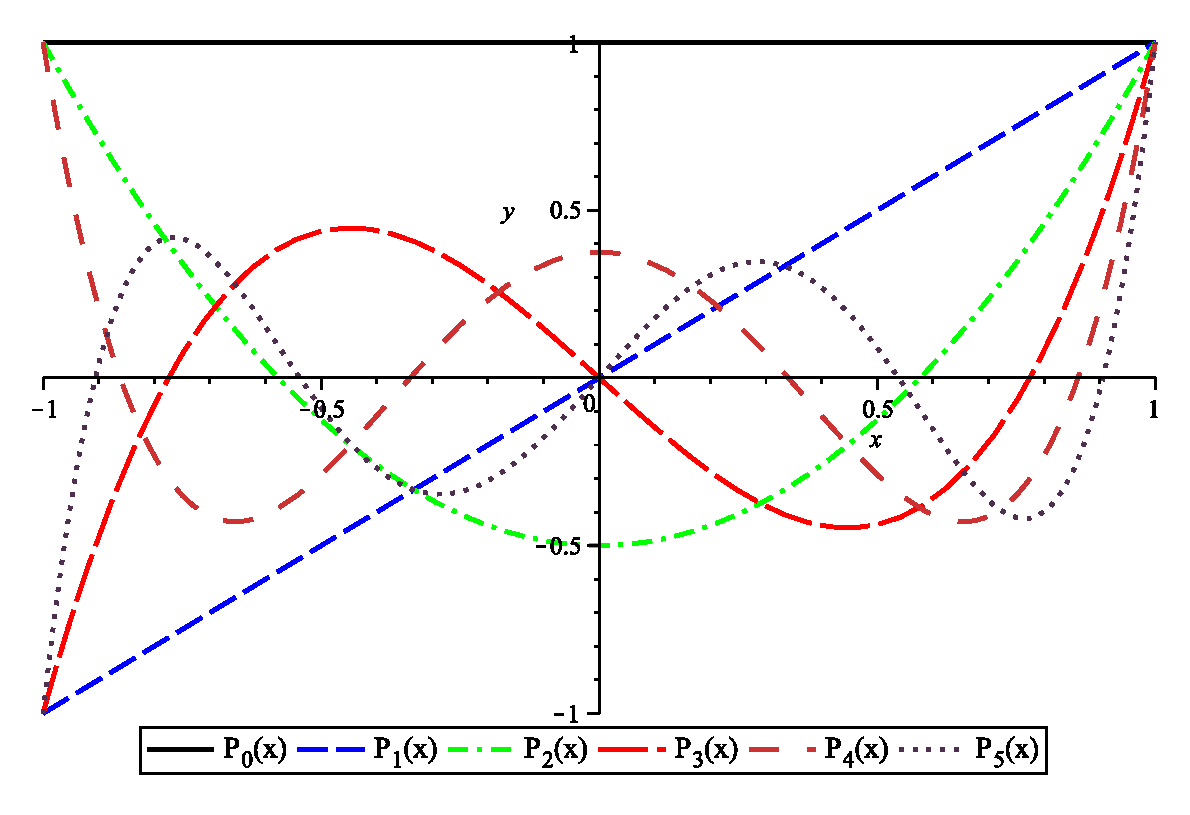
\includegraphics[keepaspectratio, width = 5.0 in]{images/legendre_polynomials}
    \caption{The first several Legendre polynomials, $P_N(x)$.}
    \label{fig:legendre_polynomials}
\end{figure}

The Legendre polynomials are useful for expanding the scattering cross-section because they are orthogonal over the range $-1 \leq \mu \leq 1$.  Moreover, expansions in the Legendre polynomials are unique in that the zeroth moment $\Sigma_{s0}$ preserves the integral properties of the underlying distribution (i.e the mean), whereas the other moments merely provide shape.  By looking at the $P_N$ in Figure \ref{fig:legendre_polynomials}, this becomes more obvious when one notes only $P_0$ has a non-vanishing integral over the domain.

\section*{Expanding the Angular Dependence}

To derive the $P_N$ equations, we must be careful to choose a starting point consistent with our expansion of the scattering kernel defined by Eqs. \ref{eq:scatterkernel} and \ref{eq:scattermoment}.  If we're not, it's easy to encounter a phantom $2\pi$!  Take as our starting point the monoenergetic transport equation in slab geometry with arbitary angular dependence of the scattering and source terms,
\begin{equation}
\begin{split}
 \mu \frac{\partial \psi}{\partial x} + \Sigma_t(x)\psi(x,\mu) &= \int^{2\pi}_0 d\phi' \int^1_{-1} d\mu' \Sigma_s(x,\mu_0)\psi(x,\mu')  + S(x,\mu)  .
\end{split}
 \label{eq:slabtransportequationgeneral}
\end{equation}

We expand the source
\begin{equation}
 S(x,\mu) = \sum^{\infty}_{n=0} \frac{2n+1}{4\pi} S_{n}(x)P_{n}(\mu) \, , 
 \label{eq:sourceexp}
\end{equation}
where
\begin{equation}
 S_{n}(x) = 2\pi \int^{1}_{-1} S(x,\mu) P_n(\mu) d\mu \, ,
\end{equation}
and the angular flux
\begin{equation}
 \psi(x,\mu) = \sum^{\infty}_{n=0} \frac{2n+1}{4\pi} \psi_{n}(x)P_{n}(\mu) \, , 
 \label{eq:psiexp}
\end{equation}
where
\begin{equation}
 \psi_{n}(x) = 2\pi \int^{1}_{-1} \psi(x,\mu) P_n(\mu) d\mu \, .
\end{equation}
% Substituting Eqs. \ref{eq:sourceexp} and \ref{eq:psiexp} along with Eq. \ref{eq:scatterkernel} into Eq. \ref{eq:slabtransportequationgeneral}, we find
% \begin{equation}
%  \begin{split}
%    & \mu \sum^{\infty}_{n=0} \frac{2n+1}{4\pi}P_{n}(\mu) \Big ( \frac{\partial \psi_n(x)}{\partial x} + \Sigma_t(x)\psi_n(x) \Big ) =  \sum^{\infty}_{n=0} \frac{2n+1}{4\pi} S_{n}(x)P_{n}(\mu) + \\
%    & \int^{2\pi}_0 d\phi' \int^1_{-1} d\mu'  \sum^{\infty}_{l=0} \frac{2l+1}{4\pi} \Sigma_{sl}P_{l}(\mu_0) \sum^{\infty}_{n=0} \frac{2n+1}{4\pi} \psi_{n}(x)P_{n}(\mu')    .
%  \end{split}
% \end{equation}
Before substituting these expressions, it helps to simplify the scattering expression.  Using Eq. \ref{eq:scatterkernel}, we can write the scattering term of Eq. \ref{eq:slabtransportequationgeneral}
\begin{equation}
\begin{split}
  \int^{2\pi}_0 d\phi' \int^1_{-1} d\mu'  & \Sigma_s(x,\mu_0)\psi(x,\mu')  \\
  &= \int^{2\pi}_0 d\phi' \int^1_{-1} d\mu'  \sum^{\infty}_{l=0} \frac{2l+1}{4\pi} \Sigma_{sl}(x)P_{l}(\mu_0) \psi(x,\mu') \, .
\end{split}
\end{equation}
Here, we make use of the \textit{Legendre addition theorem}, which states 
\begin{equation}
 P_l(\mu_0) = P_l(\mu)P_l(\mu') + 2\sum^l_{m=1}\frac{(l-m)!}{(l+m)!}P^m_l(\mu)P^m_l(\mu')\cos(m(\phi-\phi')) \, ,
\end{equation}
where $P^m_l(\mu)$ are the \textit{associated Legendre polynomials}, defined
\begin{equation}
 P^m_l(\mu) = \sqrt{(1-\mu^2)^m} \frac{d^m P_l}{d\mu^m} \, .
\end{equation}
Substituting this in, we find
\begin{equation}
\begin{split}
   \int^{2\pi}_0 d\phi' \int^1_{-1} d\mu'  & \sum^{\infty}_{l=0} \frac{2l+1}{4\pi}  \Sigma_{sl}(x)P_{l}(\mu_0) \psi(x,\mu') \\
  = \sum^{\infty}_{l=0} \frac{2l+1}{4\pi} & \Sigma_{sl}(x) \int^1_{-1} d\mu'  \psi(x,\mu')   \int^{2\pi}_0 d\phi' \Bigg ( P_l(\mu)P_l(\mu') + \\  
  & 2\sum^l_{m=1}\frac{(l-m)!}{(l+m)!}P^m_l(\mu)P^m_l(\mu')\cos(m(\phi-\phi'))\Bigg )\, .
\end{split}
\end{equation}
Noting that $ \int^{2\pi}_{0} \cos(m(\phi-\phi')) d\phi' = 0$, we find
 \begin{equation}
\begin{split}
   \int^{2\pi}_0 d\phi' \int^1_{-1} d\mu'  & \sum^{\infty}_{l=0} \frac{2l+1}{4\pi}  \Sigma_{sl}(x)P_{l}(\mu_0) \psi(x,\mu') \\
  = \sum^{\infty}_{l=0} \frac{2l+1}{4\pi} & \Sigma_{sl}(x) \int^1_{-1} d\mu'  \psi(x,\mu')   \int^{2\pi}_0 d\phi' \Big ( P_l(\mu)P_l(\mu') \Big ) \\
  = \sum^{\infty}_{l=0} \frac{2l+1}{4\pi} & \Sigma_{sl}(x)  P_l(\mu) \Bigg( 2\pi \int^1_{-1} d\mu'  \psi(x,\mu') P_l(\mu')\Bigg )  \\
  = \sum^{\infty}_{l=0} \frac{2l+1}{4\pi} & \Sigma_{sl}(x)  P_l(\mu) \psi_l(x)  \, .
\end{split}
\label{eq:simplescatter}
\end{equation}

Substituting the simplified scattering term of Eq. \ref{eq:simplescatter} and the expansions of Eqs. \ref{eq:sourceexp} and \ref{eq:psiexp} into Eq. \ref{eq:slabtransportequationgeneral} yields
\begin{equation}
 \begin{split}
   \sum^{\infty}_{n=0} &\frac{2n+1}{4\pi}P_{n}(\mu)  \Big (  \mu\frac{\partial \psi_n(x)}{\partial x} + \Sigma_t(x)\psi_n(x) \Big ) = \\
    & \sum^{\infty}_{n=0} \frac{2n+1}{4\pi}  \Sigma_{sn}(x)  P_n(\mu) \psi_n(x) + \sum^{\infty}_{n=0} \frac{2n+1}{4\pi} S_{n}(x)P_{n}(\mu) \, .
 \end{split}
 \label{eq:pnalmost}
\end{equation}
By rearranging the Legendre recurrence relation of Eq. \ref{eq:legpolyrecur}, we can express the product $\mu P_n(\mu)$ as
\begin{equation}
 \mu P_n(\mu) = \frac{1}{2n+1}\Big ( (n+1)P_{n+1}(\mu) + n P_{n-1}(\mu)\Big )\, .
\end{equation}
Substituting this in for $\mu P_n$ in the first term on the left of Eq. \ref{eq:pnalmost} and cancelling a few like terms yields
\begin{equation}
 \begin{split}
   \sum^{\infty}_{n=0} & \Bigg ( \Big ( (n+1)P_{n+1}(\mu) + nP_{n-1}(\mu) \Big )  \frac{\partial \psi_n(x)}{\partial x} + (2n+1)P_n(\mu) \Sigma_t(x)\psi_n(x) \Bigg ) = \\
    & \sum^{\infty}_{n=0} (2n+1) \Sigma_{sn}(x)  P_n(\mu) \psi_n(x) + \sum^{\infty}_{n=0} (2n+1)S_{n}(x)P_{n}(\mu) \, .
 \end{split}
 \label{eq:pnalmost2}
\end{equation}
To exploit the orthogonality property defined in Eq. \ref{eq:legpolyorth}, we multiply both sides of Eq. \ref{eq:pnalmost2} by $\frac{2m+1}{2}P_m$ and integrate the result over $-1 \leq \mu \leq 1$.  Then we find
\begin{equation}
 \begin{split}
   \int^{1}_{-1} d\mu \Bigg \{ \sum^{\infty}_{n=0} & \frac{2m+1}{2}P_m(\mu)\Bigg ( \overbrace{(n+1)P_{n+1}(\mu)\frac{\partial \psi_n}{\partial x}}^{\delta_{n+1,m}\to n=m-1} + \overbrace{nP_{n-1}(\mu)\frac{\partial \psi_n}{\partial x}}^{\delta_{n-1,m}\to n=m+1} \Bigg )   \Bigg \} = \\
   & m\frac{\partial \psi_{m-1}}{\partial x} + (m+1)\frac{\partial \psi_{m+1}}{\partial x} \, ,
 \end{split}
 \label{eq:pnalmost3a}
\end{equation}
and
\begin{equation}
 \int^{1}_{-1} d\mu \frac{2m+1}{2}P_m(\mu) (2n+1)P_n(\mu) \Sigma_t(x)\psi_n(x)  = (2m+1) \Sigma_t(x) \psi_m(x) \, ,
\end{equation}
and similarly for the scattering and source terms.  Together, we have
\begin{equation}
\begin{split}
 \frac{m+1}{2m+1}\frac{\partial \psi_{m+1}}{\partial x} &+ \frac{m}{2m+1}\frac{\partial \psi_{m-1}}{\partial x} +  \Sigma_t(x) \psi_m(x) = \\
  & \Sigma_{sm}(x) \psi_m(x) + S_m(x) \, , \, \, m = 0 \ldots \infty \, ,
\end{split}
\label{eq:pninfinite}
\end{equation}
where we take $\psi_{-1} = 0$.

\section*{The $P_N$ Equations}

Eq. \ref{eq:pninfinite} is an infinite set of coupled differential equations that represents an exact treatment in angle.  To yield a tractable problem, we make the $P_N$ approximation:
\begin{equation}
 \frac{d\psi_{N+1}}{dx} = 0 \, .
 \label{eq:pnapprox}
\end{equation}
As an example, the $P_1$ approximation yields
\begin{equation}
 \begin{split}
  n &= 0: \, \, \, \, \frac{d\psi_1}{dx} + \Sigma_t(x)\psi_0 (x) = \Sigma_{s0}\psi_0 + S_0 \\
  n &= 1: \, \, \, \, \frac{1}{3}\frac{d\psi_0}{dx} + \Sigma_t(x)\psi_1 (x) = \Sigma_{s1}\psi_1 + S_1 \, ,
 \end{split}
 \label{eq:p1approx}
\end{equation}
which is a set of two equations in the two unknown Legendre moments $\psi_0$ and $\psi_1$.  In general, the $P_N$ approximation gives $N+1$ equations in an equal number of unknowns.

An interesting fact is that the $P_N$ approximation is equalivalent to the $S_{N+1}$ approximation in slab geometry if the Gauss-Legendre quadrature set is used, proof of which is left as an exercise for the simple case of the $P_1$ and $S_2$ equations.  A similar equivalence can me made in certain cases for higher dimensions between the spherical harmonics equations and multidimensional $S_N$ approximations.  Doing so is one way to mitigate the numerical artifacts known as ray effects common to the $S_N$ approximation.  See the references in the Further Reading.

\section*{Diffusion Theory}

The $P_N$ equations give us one formal way to derive the diffusion equation.  Suppose in Eq. \ref{eq:p1approx} that we take the source to be isotropic so that $S_1 = 0$.  Moreover, we define the first scattering momement to be $\Sigma_{s1} = \Sigma_{s0}\bar{\mu}$, where $\bar{\mu} = \int^1_{-1}d\mu \mu \Sigma_s(\mu) / \int^1_{-1} d\mu \Sigma_s(\mu)$.

Then, we rearrange Eq. \ref{eq:p1approx} to find
\begin{equation}
 \psi_1 (x) = \frac{-1}{3(\Sigma_t - \Sigma_{s0}\mu)} \frac{d\psi_0}{dx} \equiv -D(x) \frac{\psi_0}{dx} \, ,
\end{equation}
so that 
\begin{equation}
 -\frac{d}{dx} D(x) \frac{\psi_0}{dx} + (\Sigma_t - \Sigma_{s0})\psi_0(x) = S_0 (x) \, .
\label{eq:neutrondiffusion}
\end{equation}
This is the diffusion equation, and we recognize $\psi_0(x)$ as the scalar flux $\phi(x)$, $\psi_1(x)$ as the current density $J(x)$, and $D$ as the diffusion coefficient.  Note that while diffusion theory explicitly assumes an isotropic source, it does treat linearly anisotropic scattering exactly.

\section*{Boundary Condition}

In general, there are two approaches to defining boundary conditions for the $P_N$ (or diffusion) equations:
\begin{enumerate}
 \item conserve net current (Marshak)
 \item obtain correct boundary flux for a finite number of $\mu$ values (Mark)
\end{enumerate}
The $P_N$ approximation consists of $N+1$ equations, which requires $N+1$ boundary conditions.  Typically, it's desirable to spread these conditions evenly among surfaces.  For a slab system, there are just two surfaces, and for odd $N$, there are an even number of conditions to be satisfied.  Hence, we typically only use odd $N$ approximations.

\section*{Marshak Conditions}

The \textit{Marshak} condition places a limit on the odd moments of the $P_N$ expansion, as the odd moments drive net flows in angular space.   Suppose we are given an incident boundary condition $B_L(\mu)$ on the left hand side, represented as
\begin{equation}
 \psi(x_L,\mu) = B_L(\mu) \, , \,\,\, \mu > 0 \, .
\end{equation}
Then the Marshak condition states
\begin{equation}
 \int^1_0 \psi(x_L,\mu)P_l(\mu)d\mu = \int^1_0 B_L(\mu) P_l(\mu)d\mu  \, ,
\end{equation}
for $l = 1,\, 3,\, \ldots \, ,N$.  In general, the Marshak conditions give the best results for the $P_N$ equations.  Moreover, they capture the physically appealing notion of conservation of particles across the boundary.

\section*{Mark Condition}

The Mark condition can be expressed as
\begin{equation}
 \psi_l(x_L) = \int^1_{-1} B_L(\mu) \delta(\mu-\mu_n)P_l(\mu) d\mu = B(\mu_n) P_l(\mu_n) \, ,
\end{equation}
for a desired set of $\mu_n$.  Typically, these $\mu_n$ are chosen to be symmetric for an equal number of $\mu_n$ per half-space.   A common choice are the $\mu_n$ such that $P_{N+1}(\mu_n) = 0$, which should look strikingly similar to the condition for generating abscissa for the Gauss-Legendre quadrature set.

\section*{A Simple Code}
To be continued.

\section*{Further Reading}
To be continued.

\begin{exercises}

  \item  \textbf{P$_{\mathbf{1}}$ Boundary Conditions}. Derive the $P_1$ equations for isotropic scattering and an isotropic source.  Derive the Marshak vacuum conditions for arbitrary left and right boundaries in a slab.  Do the same for the Mark conditions. 

  \item \textbf{P$_{\mathbf{2}}$ Equations}. Show for the case of linearly anisotropic scattering and isotropic source that the $P_2$ equations can be written as a second order partial differential equation similar in form to the typical neutron diffusion equation.

  \item \textbf{Numerical Solution of the P$_{\mathbf{1}}$ Equations}. Consider a slab of width 10 cm with $\Sigma_t = 1.0$ [cm$^{-1}$], and $c = \Sigma_s / \Sigma_t = 0.5$ (isotropic scattering in the lab system).  A uniform, isotropic source of $1$ [n/cm$^2$-s] is located in the first half of the slab, and both slab edges are subject to vacuum conditions. Write a code to solve the $P_1$ approximation to this problem using Marshak conditions.  Plot $\psi(x,\mu)$ at $x = 0$, $2.5$, $5.0$, $7.5$, and $10$ [cm].  Plot $\phi(x)$ over the whole slab.

  \item \textbf{Numerical Solution of the P$_{\mathbf{3}}$ Equations}. For the same problem, write a code to solve the $P_3$ approximation using Marshak conditions.

  \item \textbf{ Diffusion via asymptotics}.  Consider the following rescaling of the 1-d, mono-energetic transport equation with isotropic scattering. Finish me.

  \item \textbf{Legendre Addition Theorem}. Prove the Legendre polynomial addition theorem.  You may use any resource you want, but make sure you understand all steps of the proof.  A particularly straightforward approach begins as follows.  Start with an expansion of an arbitrary function in the full spherical harmonics.  Then, substitute the definition of the expansion coefficients back into the expansion.  Noting that the integral and summation can be switched, what function must the summation be?  

  \item \textbf{Defining the Scattering Angle}. Prove $\mu_0 = \cos(\theta)\cos(\theta')+\sin(\theta)\sin(\theta')\cos(\phi-\phi')$, where $\mu_0$ is the cosine of the scattering angle and ($\theta$,$\phi$) and $(\theta',\phi')$ are the original and final angles, respectively.  Include a diagram.

\end{exercises}

\chapter[Linearity and Reciprocity]{Linearity of the Transport Equation and Reciprocity Relations}

\chapter{The Adjoint and Perturbation Theory}
\label{lec:adjoint}

In this lecture, we introduce the \textit{ adjoint} form of the transport equation and describe what it represents physically.  We then apply the adjoint equation in a useful technique known as \textit{first order} or \textit{linear perturbation theory}.  In the next lecture, we make further use of the adjoint in the context of variational approximations.

\section*{The Adjoint Function}

We define the \textit{ inner product} of two  functions $\phi(x)$ and $\psi(x)$ to be
\begin{equation}
  \langle \phi, \psi \rangle \equiv \int \phi(x) \psi(x) dx \, ,
\end{equation}
where $\phi$ and $\psi$ satisfy appropriate continuity and boundary conditions.  A \textit{self-adjoint} operator $M$ satisfies
\begin{equation}
  \langle \phi, M \psi \rangle \equiv  \langle M \phi, \psi \rangle  \, .
\end{equation}
As an example, the operator corresponding to one-speed diffusion can be shown to be self-adjoint, an exercise left to the reader.  Note, self-adjoint and \textit{hermitian} are synonymous.  You may be familiar with the latter term from quantum physics, and you might recall that such operators (say the Hamiltonian) have real eigenvalues (like the energy) and orthogonal eigenfunctions (such as the nice sines and cosines of the infinite well).

If an operator $L$ is not self-adjoint, it is possible to define an operator $L^*$ that is adjoint to $L$.  Then $L^*$ will operate on adjoint functions $\psi^*(x)$ that may satisfy different boundary conditions than those of $\psi(x)$ on which $L$ operates.  The adjoint operator $L^*$ must satisfy
\begin{equation}
  \langle \psi^*, L \psi \rangle =  \langle \psi, L^* \psi^* \rangle  \, ,
  \label{eq:adjointidentity}
\end{equation}
which we refer to as the \textit{adjoint identity} (and which is actually a special case of a generalized Green's theorem).

\section*{Transport Operator}
We now define the transport equation in operator form.  Defining the operator 
\begin{equation}
  \begin{split}
     L\psi & \equiv -\hat{\Omega} \cdot \nabla \psi(\mathbf{r},\mathbf{\Omega},E) \\
           & -\Sigma_t \psi + \int^{\infty}_{0} dE' \int_{4\pi} d\Omega' \Sigma_s(\mathbf{r},\mathbf{\Omega}\cdot\mathbf{\Omega}',E'\to E)\psi(\mathbf{r},\mathbf{\Omega'},E') \, ,
  \end{split}
  \label{eq:transportoperator}
\end{equation}
the transport equation is simply $L \psi = -Q$, for some source $Q$; note the sign of the right hand side.  The transport operator $L$ is \textit{not self-adjoint}.  Convince yourself that this is indeed the case by evaluating the adjoint identity and paying specific attention to the terms corresponding to streaming and scattering.  For convenience, we assume $\psi$ is also subject to vacuum conditions on all external surfaces, i.e. $\psi(\mathbf{r},\mathbf{\Omega},E)=0$ for $\hat{n}\cdot \hat{\Omega} < 0$ where $\hat{n}$ is the outward normal vector.

The adjoint transport operator $L^*$ will satisify $\langle \psi^*, L \psi \rangle =  \langle \psi, L^* \psi^* \rangle $, if and only if we define it such that
\begin{equation}
  \begin{split}
     L^*\psi^* & \equiv \hat{\Omega} \cdot \nabla \psi^*(\mathbf{r},\mathbf{\Omega},E) \\
               & -\Sigma_t \psi^* + \int^{\infty}_{0} dE' \int_{4\pi} d\Omega' \Sigma_s(\mathbf{r},\mathbf{\Omega}\cdot\mathbf{\Omega}',E\to E')\psi^*(\mathbf{r},\mathbf{\Omega'},E') \, ,
   \end{split}
   \label{eq:adjointoperator}
\end{equation}
with the further restriction that $\psi^*(\mathbf{r},\mathbf{\Omega},E)=0$ for $\hat{n}\cdot \hat{\Omega} > 0$. It's worth noting we could have chosen conditions other than vacuum boundaries for $\psi$, which would yield different conditions for $\psi^*$; see the exercises for the case of reflecting boundaries.

\section*{Interpreting the Adjoint}

Let's consider a subcritical, time-independent system containing an arbitrary source.  Suppose we are interested in a detector response with an associated cross-section $\Sigma_d(\mathbf{r},E)$.  Then we have the forward equation
\begin{equation}
  \begin{split}
     &\hat{\Omega} \cdot \nabla \psi(\mathbf{r},\mathbf{\Omega},E) + \Sigma_t \psi = \\
     &\int^{\infty}_{0} dE' \int_{4\pi} d\Omega' \Sigma_s(\mathbf{r},\mathbf{\Omega}\cdot\mathbf{\Omega}',E'\to E)\psi(\mathbf{r},\mathbf{\Omega'},E') + Q(\mathbf{r},\mathbf{\Omega},E)  \, ,
  \end{split}
  \label{eq:foreq}
\end{equation}
subject to vacuum conditions, and the adjoint equation
\begin{equation}
  \begin{split}
     -&\hat{\Omega} \cdot \nabla \psi^*(\mathbf{r},\mathbf{\Omega},E) + \Sigma_t \psi^* = \\
     &\int^{\infty}_{0} dE' \int_{4\pi} d\Omega' \Sigma_s(\mathbf{r},\mathbf{\Omega}\cdot\mathbf{\Omega}',E\to E')\psi^*(\mathbf{r},\mathbf{\Omega'},E')  \, ,
  \end{split}
  \label{eq:adjeq}
\end{equation}
subject to the appropriate conditions.  Here, the detector cross-section, which can be thought of as a ``detector response function'', is the adjoint source.  Now, we multiply Eq. \ref{eq:foreq} by $\psi^*$ and Eq. \ref{eq:adjeq} by $\psi$, subtract the latter from the former, and integrate over all variables to get (operator and inner-product notation)
\begin{equation}
 \langle \psi^*, L \psi \rangle - \langle \psi, L^* \psi^* \rangle = - \langle \psi^*, Q \rangle +  \langle \psi, \Sigma_d \rangle \, ,
\end{equation}
but by the adjoint identity, the left hand side vanishes, and we are left with a most important result:
\begin{equation}
 \langle \psi^*, Q \rangle =  \langle \psi, \Sigma_d \rangle \, .
 \label{eq:adjrule}
\end{equation}
Suppose our forward source is a unit monoenergetic, unidirectional point source, i.e. $Q(\mathbf{r},\mathbf{\Omega},E) = \delta(\mathbf{r}-\mathbf{r}_0)\delta(\mathbf{\Omega}-\mathbf{\Omega}_0)\delta(E-E_0)$.  From Eq. \ref{eq:adjrule}, we find
\begin{equation}
 \psi^*(\mathbf{r}_0,\mathbf{\Omega}_0,E_0) = \int_V d^3r \int_{E} dE \int_{4\pi} d\Omega \Sigma_d(\mathbf{r},E') \psi(\mathbf{r},\mathbf{\Omega},E) = R \, ,
\end{equation}
where $R$ is the total detector response.  In this case, $\psi^*(\mathbf{r}_0,\mathbf{\Omega}_0,E_0)$ is the expected contribution to the detector response due to a unit delta source located at $(\mathbf{r}_0,\mathbf{\Omega}_0,E_0)$ in phase space.  More broadly, $\psi^*$ represents the importance of neutrons in a particular region of phase space to a given detector response.

\section*{Perturbation Theory --- Fixed Source}

In this and the next section, we apply the adjoint in determining the change to an integral system parameter\footnote{Here, an ``integral'' parameter is any integrated quantity, e.g. a reaction rate in a volume, or $k_{e\!f\!f}$ in a reactor.} due to a small perturbation in the system.  We begin with a fixed source example and follow with an eigenvalue example.

Suppose we have a system described by\footnote{Note, the operators in this section have absorbed the minus sign of the right hand side sources above.}
\begin{equation}
 L_0 \psi_0 = Q_0 \, 
\end{equation}
with vacuum boundaries.  Our goal is to evaluate a detector response that takes the form
\begin{equation}
 R_0 = \int \int \int d^3r d\Omega dE \Sigma_d(\mathbf{r},E) Q(\mathbf{r},E,\mathbf{\Omega}) \, .
\end{equation}

Suppose we now introduce some small change.  Perturbation theory can allow us to determine the detector response, to first order accuracy, for a ``small'' perturbation to the system.  Let us define a new, perturbed system to be
\begin{equation}
 L \psi = Q \, ,
\end{equation}
also subject to vacuum conditions, and where $L = L_0 + \delta L_0$, $Q = Q_0 + \delta Q_0$, and $\psi = \psi_0 + \delta \psi_0$.  We assume we know $L$ and $Q$ (we're making the perturbation), and we want to know $\psi$ (and eventually, its effect on $R$). Rewriting the system, we have
\begin{equation}
\begin{split}
 ( L_0 + \delta L_0)(\psi_0 + \delta \psi_0) &= Q_0 + \delta Q_0 \\
  L_0 \psi_0 + \delta L_0 \psi_0 + L_0 \delta \psi_0 + \theta(\delta^2) &= Q_0 + \delta Q_0 \, ,
\end{split}
\end{equation}
but noting our original equation is contained, we are left with two separate equations,
\begin{equation}
 L_0 \psi_0 = Q_0 \, ,
 \label{eq:pertzeroth}
\end{equation}
and
\begin{equation}
 \delta L_0 \psi_0 + L_0 \delta \psi_0 = \delta Q_0 \, ,
 \label{eq:pertfirst}
\end{equation}
where we have neglected terms of order $\delta^2$; hence the theory is known as ``first order'' or ``linear'' perturbation theory.

We now introduce the adjoint to the \textit{original equation}, with the adjoint source being our detector response function $\Sigma_d$, i.e.
\begin{equation}
 L^*_0 \psi^*_0 = \Sigma_d \, ,
 \label{eq:pertadj}
\end{equation}
and as before, we have $\langle \psi^*_0, Q_0 \rangle =  \langle \psi_0, \Sigma_d \rangle = R_0$.  Our goal is to determine $\delta R_0$, or $R-R_0 = \delta R_0 =  \langle \delta \psi_0, \Sigma_d \rangle$.  To do so, we multiply Eq. \ref{eq:pertfirst} by $\psi^*_0$ and Eq. \ref{eq:pertadj} by $\delta \psi_0$, subtract the latter from the former, and integrate over all phase space, yielding
\begin{equation}
  \langle \psi^*_0, \delta L_0 \psi_0 \rangle + \langle \psi^*_0, L_0 \delta \psi_0 \rangle - \langle L^*_0 \psi^*_0, \delta \psi_0 \rangle = \langle \psi^*_0, \delta Q_0 \rangle - \langle \delta \psi_0, \Sigma_d \rangle \, .
\end{equation}
The second and third terms on the left hand side cancel by way of the adjoint identity, and the second term on the right hand side is $\delta R_0$.  Thus, we have
\begin{equation}
 \delta R_0 = \langle \psi^*_0, \delta Q_0 \rangle - \langle \psi^*_0, \delta L_0 \psi_0 \rangle \, .
 \label{eq:fixedpertresp}
\end{equation}
From Eq. \ref{eq:fixedpertresp}, we see that an increased source gives rise to a \textit{greater} response, and an increase in $L$, corresponding to greater leakage or interaction, produces a \textit{lower} response, as is expected.

\section*{Perturbation Theory --- Eigenvalue}

As another example of perturbation theory, consider the unperturbed eigenvalue problem
\begin{equation}
 H_0 \psi_0 = \lambda_0 F_0 \psi_0 \, 
\end{equation}
subject to vacuum conditions.  As above, suppose we introduce some small change, and let a new, perturbed system be
\begin{equation}
  H \psi = \lambda F \psi \, .
\end{equation}
where $H = H_0 + \delta H_0$, $F = F_0 + \delta F_0$, $\psi = \psi_0 + \delta \psi_0$, and $\lambda =\lambda_0 + \delta \lambda_0$.  Our goal is to find $\delta \lambda_0$ due to the perturbation.  

We rewrite the perturbed system
\begin{equation}
 (H_0 + \delta H_0)(\psi_0 + \delta \psi_0) = (\lambda_0 + \delta \lambda_0)(F_0 + \delta F_0)(\psi_0 + \delta \psi_0) 
\end{equation}
and expand
\begin{equation}
\begin{split}
  H_0 \psi_0 + \delta H_0 \psi_0 &+ H_0 \delta \psi_0 + \theta(\delta^2) \\
      &= \lambda_0 F_0 \psi_0 + \lambda_0 F_0 \delta \psi_0 + \lambda_0 \delta F_0 \psi_0 + \delta \lambda_0 F_0 \psi_0 + \theta(\delta^2)  \, .
\end{split}
\end{equation}
Again, we recognize our original equation and a second equation with first-order perturbations,
\begin{equation}
 (H_0 - \lambda_0 F_0) \delta \psi_0 = (\lambda_0 \delta F_0 \psi_0 ) - (\delta H_0 - \delta \lambda_0 F_0)\psi_0 \, .
 \label{eq:eigenpertfirst}
\end{equation}

We define the adjoint problem
\begin{equation}
 H^*_0 \psi^*_0 = \lambda_0 F^*_0 \psi^*_0 \, 
 \label{eq:eigenpertadj}
\end{equation}
subject to the appropriate boundary conditions.  Similar to our treatment in the fixed source example, we multiply Eq. \ref{eq:eigenpertfirst} by $\psi^*_0$ and Eq. \ref{eq:eigenpertadj} by $\delta \psi_0$, subtract the latter from the former, and integrate over all phase space.  After a bit of rearranging, we find
\begin{equation}
 \delta \lambda_0 = \frac{\langle \psi^*_0,(\delta H_0 - \lambda_0 \delta F_0)\psi_0 \rangle}{\langle \psi^*_0, F_0 \psi_0 \rangle} \, .
 \label{eq:eigenpertresp}
\end{equation}

\section*{Further Reading}

Most of the development here follows that of Bell and Glasstone \cite{bell1970nrt}, Chapter 6.  Duderstadt and Hamilton \cite{duderstadt1976nra} develop the adjoint within the diffusion framework and apply it to problems of reactor physics in Chapters 5 and 7.  A particularly appealing description of the physical interpretation of the adjoint, albeit with a reactor physics flavor, is given by Henry \cite{henry1975nra}.  

It's worth noting that the adjoint was developed first by Lagrange as a mathematical construct; however, its physical utility was first realized much later in the context of quantum mechanical perturbation theory, and later yet in reactor physics.  This history and more is to be found in Marchuk's treatise on adjoint methods \cite{marchuk1995aea}.  That first application of the adjoint in reactor physics was due to the ``father of nuclear engineering,'' Eugene Wigner \cite{wigner1945esp}.  

The available literature on perturbation theory is quite large.  One important recent effort has been to couple sensitivities defined by perturbation theory to cross-section uncertainties in order to estimate the uncertainty of integral system parameters including the eigenvalue \cite{broadhead2004sau} and various worths \cite{williams2007sau} due to the underlying data uncertainty.  

\begin{exercises}

  \item \textbf{Self-adjointness}. Prove the one-speed diffusion operator, i.e. $L\phi = D\phi_{xx} - \Sigma_a\phi(x) = -S$ is self-adjoint.  You may assume a homogeneous medium with zero-flux boundary conditions, neglecting extrapolation distances.

  \item \textbf{Adjoint Transport Equation}. Demonstrate that the adjoint operator $L^*$ defined by Eq. \ref{eq:adjointoperator} really is the adjoint to the forward operator $L$ for the given boundary conditions.

  \item \textbf{Adjoint Boundary Conditions}. (a) For the case that $\psi$ satisfies vacuum conditions, we found that $\psi^*(\mathbf{r},\mathbf{\Omega},E)=0$ for $\hat{n}\cdot \hat{\Omega} > 0$.  What does this mean physically?  (b) For the one-speed transport equation, derive the boundary conditions for $\psi^*$ when $\psi$ satisfies reflecting conditions.

  \item \textbf{Using the Adjoint}. (a) Briefly describe the physical meaning of the adjoint flux. (b) Suppose we have a known shield with a known detector on one side.  Suppose further that the particle source on the opposite side of the shield is not known \textit{a priori} and can take widely varying forms.  (An example of this might be a shielding analysis for a fusion reactor, where we think we have a good shield and then we try using it for several possible sources).  How could the adjoint be used so that only one ``transport'' calculation would be needed to compute the detector dose given an arbitrary source?

  \item \textbf{A Point Detector}. Repeat the process used to obtain $\psi^* = R$ but for the case of a point detector, $\Sigma_d = \delta(\mathbf{r}-\mathbf{r}_0)\delta(\mathbf{\Omega}-\mathbf{\Omega}_0)\delta(E-E_0)$.  Clearly, one obtains an expression for $\psi(\mathbf{r}_0,\mathbf{\Omega}_0,E_0)$.  What does $\psi^*(\mathbf{r},\mathbf{\Omega},E)$ represent in this case?  This result is a generalization of reciprocity relations previously discussed for one-speed transport.

  \item \textbf{The ``Contributon'' Flux}. In 1-d and one-speed, define the quantity 
  \begin{equation*}
   C(x,\mu) = \psi(x,\mu)\psi^*(x,\mu) \, ,
  \end{equation*}
  where $\psi$ and $\psi^*$ are the forward and adjoint angular fluxes.  Take the forward problem to have vacuum boundaries.  (a) Mathematically, express the vacuum boundary condition for $\psi$ at a general external boundary $x_b$.  (b) With your knowledge of the corresponding adjoint boundary condition, write down the mathematical expression for the boundary condition of $C(x,\mu)$.  (c) Taking the adjoint source to be a flux-to-dose factor, what are the units of $\psi$, $\psi^*$, and $C$?  Can you interpret $C$ physically?  (For more information on this mysterious quantity, see the paper by Williams \cite{williams1991gcr}.)

  \item \textbf{Eigenvalue Perturbation}.  Prove Eq. \ref{eq:eigenpertresp}.  Also, describe what possible changes in the system coincide with the perturbations $\delta H_0$ and $\delta F_0$ and how such changes impact the eigenvalue perturbation.  Remember that $k_{e\!f\!f}$ is $\lambda^{-1}$.

  \item \textbf{Eigenvalue Sensitivity}.  Defining the sensitivity of $k_{e\!f\!f}$ to a cross-section $\Sigma_x$ to be
  \begin{equation*}
   S_{k,\Sigma_x} = \frac{\Sigma_x}{k_{e\!f\!f} }\frac{\partial k_{e\!f\!f}}{ \partial \Sigma_x} \, ,
  \end{equation*}
  find an expression for $S_{k,\Sigma_x}$ in terms of the partial derivatives of $H_0$ and $F_0$ with respect to $\Sigma_x$.


\end{exercises}

\chapter{Variational Methods}

In this lecture, we investigate use of \textit{variational principles} in the 
context of nuclear engineering.  An entire course could be devoted to this 
subject; here, we focus on the same two quantities analyzed in 
Lecture \ref{lec:adjoint}, namely the reaction rate for a fixed source problem 
and the eigenvalue of an eigenvalue problem.  We demonstrate that variational 
principles can be used to estimate these quantities using approximate fluxes. 
We finish by showing how our first order perturbation theory can be derived 
directly from variational principles.

\section*{Variational Principles, Functionals, and Stationary Points}

A variational principle casts a particular function, usually a problem's 
solution, as the stationary point of some \textit{functional}. Often, the 
functional itself is called the variational principle.  A functional is 
simply a function that takes another function as its argument and returns 
a scalar as its value.  Consider a function $f(x) = Ax + B$.  A possible 
functional would be $F[f(x)] = \int_{x_1}^{x_2} f(x)dx$, which certainly 
yields a scalar value.  Typically, the value of the functional represents 
a quantity of interest, which in transport applications is often a 
reaction rate.

We see that functionals are quite like functions; how exactly then do we 
define a \textit{stationary point}, and what does it mean in the context 
of a variational principle?  Recall from elementary calculus that a stationary 
point is the value of the independent variables such that the function reaches 
a local extremum (or saddle-point), i.e. the function's derivative (or 
gradient) vanishes.  The same idea applies to functionals.  Defining 
the ``weak derivative'' of $F$ at a point $f(x)$ in the direction $g(x)$ as
\begin{equation}
 \delta F[f,g] = \lim_{\epsilon \to 0} 
                 \frac{ F[f+\epsilon g] - F[f] }{\epsilon} \, ,
\end{equation}
the \textit{first variation} of $F$ is defined 
\begin{equation}
 \delta F[f,g] = \left ( \frac{d}{d\epsilon} F[f+\epsilon g] \right ) 
                 \Bigg |_{\epsilon = 0} \, ,
\end{equation}
for arbitrary $g$.  When $\delta F[\tilde{f},g] = 0$ for all $g$, $\tilde{f}$ 
is called a \textit{stationary point} of $F$, and the expression
\begin{equation}
 \delta F[\tilde{f},g] = 0 \, ,  \, \, \, \, \, \, \forall g 
\end{equation}
defines the variational principle for $\tilde{f}$.  For $F[f]$ that represents 
a quantity of interest, $F[\tilde{f}]$ represents the true value for that 
quantity.  Moreover, very near the stationary point, $\delta F \to 0$ by 
construction, and the errors in $F$ (and hence the quantity of interest) are 
second order, which gives rise to the utility of variational approximations.

\section*{A Simple, Illustrative Example}

It is easiest to understand these ideas through a simple example (unrelated 
to nuclear engineering).  Suppose we wish to find the curve giving us the 
shortest difference between two points in a plane.  Of course, this is 
intuitive: the solution should be a line.  We show this using variational 
techniques.  

Let the curve be $y(x)$. From any calculus book, we know the differential arc 
length is then
\begin{equation}
 dl = \sqrt{ dx^2 + dy^2 } = \sqrt{1 + (y')^2} \, .
\end{equation}
We take as our functional the arc length,
\begin{equation}
 F[y] = \int^{x_2}_{x_1} \sqrt{1 + (y')^2} dx \, ,
\end{equation}
where ($x_1$, $y_1$) and ($x_2$, $y_2$) are the points of interest.  

Taking the first variation of $F$,
\begin{equation}
\begin{split}
\delta F[y,g] &= \left ( \frac{d}{d\epsilon}\int^{x_2}_{x_1} 
                         \sqrt{1 + (y'(x)+\epsilon g'(x))^2} dx \right ) 
                 \Bigg |_{\epsilon=0} \\
              &= \left ( \int^{x_2}_{x_1} 
                         \frac{(y'(x)+\epsilon g'(x))g'(x)}
                              {\sqrt{1 + (y'(x)+\epsilon g'(x))^2}} \right ) 
                 \Bigg |_{\epsilon=0} \\
              &= \int^{x_2}_{x_1} \frac{y'(x)g'(x)dx}{\sqrt{1 + (y'(x))^2}} \, ,
\end{split}
\end{equation}
we find that the arc length is minimized when
\begin{equation}
 \delta F[y,g] =
   \int^{x_2}_{x_1}\frac{y'(x)g'(x)}{\sqrt{1 + (y'(x))^2}} = 0 \, .
 \label{eq:exampleprinciple}
\end{equation}
In this form, we can't say anything about $y$ or $g$.  Instead, we use 
integration by parts to go from $y'$ and $g'$ to $y''$ and $g$, and
Eq. \ref{eq:exampleprinciple} becomes
\begin{equation}
 \delta F[y,g] =
   \left [ \frac{y'(x)g(x)}{\sqrt{1 + (y'(x))^2}} \right ]^{x_2}_{x_1} - 
   \int^{x_2}_{x_1} \frac{y''(x)g(x)dx}{(1 + (y'(x))^2)^{\frac{3}{2}}} = 0\, .
 \label{eq:exampleprinciple2}
\end{equation}
While $g(x)$ is arbitrary \textit{between} $x_1$ and $x_2$, we must have 
$g(x_1) = g(x_2) = 0$ to that $y(x_1) = y_1$ and $y(x_2) = y_2$.  Thus, the 
first term of Eq. \ref{eq:exampleprinciple2} vanishes. 
By inspection, the second term vanishes for 
arbitrary $g$ only if $y'' = 0$.  This relation is known as 
the \textit{Euler equation}\footnote{In general, setting the first variation 
to zero gives rise to a set of partial differential equations collectively 
known as the Euler equations.}.  Of course, to satisfy $y''=0$ requires 
our solution $\tilde{y}(x)$ to be of the form $Ax+B$, as expected.

\section*{A Variational Principle for Fixed Source Problems}

Suppose we are interested in a linear functional of the flux, such 
as $G_{\text{fs}}[\psi] = \langle \psi, \Sigma_d \rangle$, a reaction rate. 
An appropriate variational principal is represented by 
the \textit{generalized Roussopoulos functional}
\begin{equation}
 F_{\text{fs}} [\psi,\psi^*] = G_{\text{fs}}[\psi] + \langle \psi^*, (Q-L\psi) \rangle \, .
\end{equation}
Note, $\delta F_{\text{fs}}[\psi,\psi^*] = 0$ is a variational principle 
for $G_{\text{fs}}$ if the corresponding solution $\psi$ 
yields $F_{\text{fs}}[\psi,\psi^*] = G_{\text{fs}}[\psi]$.  We see this is so when 
the second term of $F$ vanishes when $\psi$ solves $L\psi = Q$, i.e. 
when $\psi$ is the solution to the transport equation.

To determine the variational principle, we take the first variation of $F_{\text{fs}}$,
\begin{equation}
 \begin{split}
  \delta F_{\text{fs}} [\phi,\phi^*] &= 
    \left ( \frac{d}{d\epsilon} 
            \left ( \langle (\phi+\epsilon \delta \phi) \Sigma_d \rangle + 
                    \langle (\phi^* + \epsilon \delta \phi^*), 
                            (Q-L(\phi+\epsilon \delta \phi)) \rangle 
            \right ) 
    \right ) \Bigg|_{\epsilon=0} \\
   &= \langle \delta \phi, \Sigma_d \rangle - 
      \langle \phi^*,L \delta \phi \rangle + 
      \langle \delta \phi^*, Q \rangle - 
      \langle \delta \phi^*, L \phi \rangle \, .
 \end{split}
\end{equation}
Noting 
$\langle \phi^*,L\delta \phi \rangle = \langle L^* \phi^*,\delta \phi \rangle$, 
we have for our principle 
\begin{equation}
 0 = \langle \delta \phi, (\Sigma_d - L^* \phi^*) \rangle + 
     \langle \delta \phi^*, (Q-L\phi) \rangle \, ,
\end{equation}
which is satisfied when $L\phi = Q$ and $L^* \phi^* = \Sigma_d$.  These are 
the corresponding Euler equations, and we see they are just the original 
forward and adjoint transport equations.

The importance of this variational principle (and others in general) is that 
it gives us an estimate for $G_{\text{fs}}$ accurate to second order for approximate 
fluxes $\phi$ and $\phi^*$.  To demonstrate this, suppose the true solutions 
to the Euler equations are $\psi$ and $\psi^*$.  
Let $\phi = \psi + \delta \psi$ and $\phi^* = \psi^* + \delta \psi^*$.  
We subsitute these expressions into $F$ and find
\begin{equation}
 \begin{split}
    F_{\text{fs}} [\phi,\phi^*] &= 
      \langle \Sigma_d, (\psi+\delta \psi) \rangle + 
      \langle (\psi^*+\delta \psi^*),(Q-L(\psi+\delta \psi^*) \rangle \\
    &= \langle \Sigma_d,\psi \rangle + 
       \langle \Sigma_d, \delta \psi \rangle + 
       \langle \psi^*,Q \rangle + 
       \langle \delta \psi,Q \rangle  \\ 
    &- \langle \psi^*, L\psi \rangle - 
       \langle \psi^*, L\delta \psi \rangle - 
       \langle \delta \psi^*, L\psi \rangle - 
       \langle \delta \psi^*, L\delta \psi \rangle \\
    &= \langle \Sigma_d, \psi \rangle - 
       \langle \delta \psi^*, L\delta \psi \rangle \\
    &= G_{\text{fs}}[\psi] + \mathcal{O}(\delta^2) \, .
 \end{split}
 \label{eq:secondorderfs}
\end{equation}
Hence, $F$ provides a first order accurate (i.e. good through first order) 
estimate of the reaction rate given approximate forward and adjoint fluxes.

\section*{A Variational Principle for Eigenvalue Problems}

For eigenvalue problems, an appropriate functional is 
the \textit{Rayleigh quotient}
\begin{equation}
 F_{\text{ev}}[\psi,\psi^*] = 
   \frac{\langle \psi^*,L\psi \rangle}{ \langle \psi^*, F \psi \rangle } \, .
 \label{eq:rayleigh}
\end{equation}
Here, the quantity of interest is $G_{\text{ev}} = \lambda$, and, unlike the 
fixed source case, we have $G_{\text{ev}} = F_{\text{ev}}$.  You should show 
that $F_{\text{ev}}$ is in fact a valid expression for $\lambda$.  The 
associated Euler equations are just the forward and adjoint eigenvalue 
equations, which can be shown by setting the first variation 
of $F_{\text{ev}}$ to zero, an exercise left to the reader.

For approximate fluxes $\phi$ and $\phi$, it can be shown that
\begin{equation}
 F_{\text{ev}}[\phi,\phi^*] = \lambda + \mathcal{O}(\delta^2) \, ,
\end{equation}
the proof of which is left as an exercise.

\section*{Perturbation Theory from Variational Principles}

In general, it is possible to find first order perturbation estimates using 
the expression
\begin{equation}
 \delta = \bar{F}[\psi,\psi^*] - F[\psi,\psi^*] \, ,
 \label{eq:pertfromvar}
\end{equation}
where $F$ is the appropriate functional with nominal operators 
and $\bar{F}$ is the function evaluated with perturbed operators.  It must 
be stressed that $\psi$ and $\psi^*$ are assumed to be the exact fluxes for 
the unperturbed problem.

As an example, we re-derive the first order perturbation to a detector 
response.  Suppose the perturbations to our system 
include $L+\delta L$, $Q+\delta Q$, 
and $\Sigma_d + \delta \Sigma_d$.  Then Eq. \ref{eq:pertfromvar}  gives
\begin{equation}
\begin{split}
 \delta_{\text{fs}} &= \bar{F}[\psi,\psi^*] - F[\psi,\psi^*] \\
        &= \langle \psi, (\Sigma_d+\delta \Sigma_d) \rangle + 
           \langle \psi^*,(Q+\delta Q-(L+\delta L)\psi ) \rangle - 
           \langle \psi, \delta \Sigma_d \rangle \\
        &= \langle \psi,\delta \Sigma_d \rangle + 
           \langle \psi^* , \delta Q \rangle - 
           \langle \psi^*,\delta L \psi \rangle \, .
\end{split}
\label{eq:fixedpertvar}
\end{equation}
The last line is equivalent to Eq. \ref{eq:fixedpertresp} with the addition 
of the first term, which explicitly accounts for changes in the detector 
response function.

Eq. \ref{eq:pertfromvar} can also be applied to the Rayleigh quotient, 
yielding Eq. \ref{eq:eigenpertresp}, proof of which is left 
as an exercise.

\section*{Further Reading}

Most of the material presented here is contained in Chapter 7 of 
Duderstadt and Martin \cite{duderstadt1976tt}  in addition to Chapter 1 
of Stacey \cite{stacey1974vmn}.  The former contains several examples 
and a variational derivation of the diffusion equation.  The reader is 
also encouraged to look up Pomraning's large body of work on variational 
methods\footnote{It is worth noting that Stacey and Pomraning, both with 
prolific work in variational methods, did their graduate work in 
this department.}.

\begin{exercises}

  %----------------------------------------------------------------------------%
  \item \textbf{Second Order Accuracy}. 
    Show that the Roussopoulos functional $F[\phi,\phi^*]$ gives a second 
    order accurate value for $\langle \psi,\Sigma_d \rangle$ when $\phi$ 
    and $\phi^*$ are approximate values of $\psi$ and $\psi^*$, i.e. 
    prove Eq. \ref{eq:secondorderfs}.

  %----------------------------------------------------------------------------%
  \item \textbf{Fixed Source Perturbation}. 
    Prove Eq. \ref{eq:fixedpertvar}.
 
  %----------------------------------------------------------------------------%
  \item \textbf{Rayleigh Quotient}. 
    \begin{enumerate}[a.]
      \item Take the first variation of the Rayleigh quotient with respect to 
            the forward and adjoint fluxes and show the stationarity conditions 
            are just the forward and adjoint eigenvalue problems. 
      \item Demonstrate that the Rayleigh quotient is a second order 
            estimator for $\lambda$.
    \end{enumerate}

  %----------------------------------------------------------------------------%
  \item \textbf{Losses-to-Gains}. 
    Directly from the eigenvalue equation, we find 
    \begin{equation*}
      \lambda = (L\psi)/(F\psi) \, ,
    \end{equation*}
    a compact way to define losses-to-gains.  
    \begin{enumerate}[a.]
      \item Show why this is not a variational principle for $\lambda$.
      \item Consider again Eq. \ref{eq:rayleigh}.  How does the adjoint change 
            the physical interpretation of gains-to-losses?
    \end{enumerate}

  %----------------------------------------------------------------------------%
  \item  \textbf{Eigenvalue Perturbation}. 
    Prove that $\bar{F}_R[\psi,\psi^+]-F_R[\psi,\psi^+]$ yields the first 
    order perturbation estimate for $\delta \lambda$ given 
    by Eq. \ref{eq:eigenpertresp}.

  %----------------------------------------------------------------------------%
  \item  \textbf{Applying Roussopoulos}. 
    Consider a 1-d, 1-speed diffusion problem in a slab of 
    width $2a$, $\Sigma_a = 0.022$, and $D = 0.14$. 
    \begin{enumerate}[a.]
      \item Solve for the exact scalar flux $\phi(x)$, using the 
            conditions $\phi(\pm a)=0$, and
            assuming a uniform source $Q(x) = 1$ and $a=1$.
      \item Compute the total absorption rate in the slab.
      \item Now, approximate the solution as 
            $\tilde{\phi}(x) = Ax^2 + Bx +C$ with the same maximum 
            and the same boundary conditions.  Compute the absorption rate  
            using $\tilde{\phi}(x)$.
      \item Finally, recalling the 1-d, 1-speed diffusion equation is 
            self-adjoint, use the Roussopoulos principle to compute the 
            absorption rate.  What can you conclude? 
    \end{enumerate}

  %----------------------------------------------------------------------------%
  \item \textbf{More Roussopoulos}. 
    For same problem, estimate the total absorption rate if something 
    causes $\Sigma_a = 1.1$.  Be careful to consider the impact of the change 
    in $\Sigma_a$ on both $\Sigma_d$ and $L$.

  %----------------------------------------------------------------------------%
  \item \textbf{Approximating Escape from a Slab}. 
    Consider the escape probability $P_{\text{esc}}$ for a homogeneous 1-d slab, 
    the subject of 
    Chapter \ref{lec:analytical}, Problem \ref{itm:escapeprobability}.  
    Here, consider a discrete ordinates approximation using the 
    two point Gauss-Legendre quadrature for a 10 cm slab 
    with $\Sigma_t = 10$ [1/cm].
    \begin{enumerate}[a.]
      \item Solve for $P_{\text{esc}}$ directly using the S$_{\text{2}}$ 
            approximation and Mark boundary conditions.  
      \item Use a variational principle to improve 
            your estimate of $P_{\text{esc}}$. 
      \item Compare both values to the exact value.
    \end{enumerate}

\end{exercises}


\part{Bibliography and Appendices} 

% Reset to a simple chapter title and format
\renewcommand\printchaptertitle[1]{%
    \begin{tabular}{@{\Large\bfseries\chaptername}@{ }p{1.0cm}!{\quad}p{\textwidth-4cm-2em-4\tabcolsep }}
      \ifNoChapNumber\relax\else\chapnumfont \thechapter\fi
      & \chaptitlefont 
    \end{tabular}
    \NoChapNumberfalse
}
\renewcommand{\chaptername}{Bibliography}
\bibliographystyle{plain}
\bibliography{biblio106}


\appendix
\renewcommand{\chaptername}{Appendix}
\chapter{Nomenclature}

To facilitate understanding of the various terms used throughout the lecture materials, we provide here a list of variables, short definitions, and common units where applicable.  In very few cases, symbols are used more than once due to convention (e.g. $\phi$ for both flux and azimuthal angle).  Bold symbols indicate a vector quantity.

\begin{table}[th]
 \caption{Fundamental quantities}
 \begin{center} 
 {\small
 \begin{tabular*}{0.90\textwidth}{@{\extracolsep{\fill}} ccc } 
  \toprule 
   Symbol                            & Description   & Units  \\
  \midrule 
   $\psi(\vec{r},\hat{\Omega},E,t)$          & angular flux                  & $\frac{\mathrm{n}}{\mathrm{cm^2-s-eV-ster}}$  \\
   $\psi^+(\vec{r},\hat{\Omega},E,t)$        & adjoint angular flux          & $\frac{\mathrm{n}}{\mathrm{cm^2-s-eV-ster}}$  \\
   $\phi(\vec{r},E,t)$                       & scalar  flux                  & $\frac{\mathrm{n}}{\mathrm{cm^2-s-eV}}$  \\
   $\phi^+(\vec{r},E,t)$                     & adjoint scalar flux           & $\frac{\mathrm{n}}{\mathrm{cm^2-s-eV}}$  \\
   $\mathbf{j}(\vec{r},\hat{\Omega},E,t)$    & angular current density       & $\frac{\mathrm{n}}{\mathrm{cm^2-s-eV-ster}}$  \\
   $\mathbf{ J}(\vec{r},E,t) $               & current density               & $\frac{\mathrm{n}}{\mathrm{cm^2-s-eV}}$  \\
   $J_{\pm}(\vec{r},E,t)$                    & partial current density       & $\frac{\mathrm{n}}{\mathrm{cm^2-s-eV}}$  \\
  \bottomrule 
 \end{tabular*} 
 }
 \end{center} 
 \label{tbl:snmeshstudy}  
\end{table}



\end{document}